% CVPR 2025 Paper Template; see https://github.com/cvpr-org/author-kit

\documentclass[10pt,twocolumn,letterpaper]{article}

%%%%%%%%% PAPER TYPE  - PLEASE UPDATE FOR FINAL VERSION
% \usepackage{cvpr}              % To produce the CAMERA-READY version
% \usepackage[review]{cvpr}      % To produce the REVIEW version
\usepackage[pagenumbers]{cvpr} % To force page numbers, e.g. for an arXiv version

% Import additional packages in the preamble file, before hyperref
%
% --- inline annotations
%
\newcommand{\red}[1]{{\color{red}#1}}
\newcommand{\todo}[1]{{\color{red}#1}}
\newcommand{\TODO}[1]{\textbf{\color{red}[TODO: #1]}}
% --- disable by uncommenting  
% \renewcommand{\TODO}[1]{}
% \renewcommand{\todo}[1]{#1}

\usepackage{xcolor}
\usepackage{graphicx}
\usepackage{booktabs}
\usepackage{amsmath} 
\usepackage{amsfonts}
\usepackage{amssymb}
\usepackage{multirow} 
\usepackage{makecell}
\newcommand{\shline}{\Xhline{1.1pt}} % Adjust thickness as desired

% It is strongly recommended to use hyperref, especially for the review version.
% hyperref with option pagebackref eases the reviewers' job.
% Please disable hyperref *only* if you encounter grave issues, 
% e.g. with the file validation for the camera-ready version.
%
% If you comment hyperref and then uncomment it, you should delete *.aux before re-running LaTeX.
% (Or just hit 'q' on the first LaTeX run, let it finish, and you should be clear).
\definecolor{cvprblue}{rgb}{0.21,0.49,0.74}
\usepackage[pagebackref,breaklinks,colorlinks,allcolors=cvprblue]{hyperref}

%%%%%%%%% PAPER ID  - PLEASE UPDATE
\def\paperID{6504} % *** Enter the Paper ID here
\def\confName{CVPR}
\def\confYear{2025}

\title{\ssm: A Recurrent Video Transformer}

%%%%%%%%% AUTHORS - PLEASE UPDATE
\author{Viorica P\u{a}tr\u{a}ucean$^{*}$ \and Xu Owen He$^{*}$ \and Joseph Heyward$^{*}$ \and Chuhan Zhang$^{*}$ \and Mehdi S.\ M.\ Sajjadi \and George-Cristian Muraru \and Artem Zholus \and Mahdi Karami \and Ross Goroshin \and Yutian Chen \and Simon Osindero \and João Carreira \and Razvan Pascanu \\[3mm]
\small{Google DeepMind} \\
\small{Corresponding author: \texttt{viorica@google.com}, $^{*}$core contributor}
}


\begin{document}
% \maketitle
\vspace{-2em}
\vspace{-2mm}
% \twocolumn[{%
% \renewcommand\twocolumn[1][]{#1}%
% \maketitle
% % \begin{figure*}[!ht]
% \begin{subfigure}{0.6\textwidth}
%     \centering
%     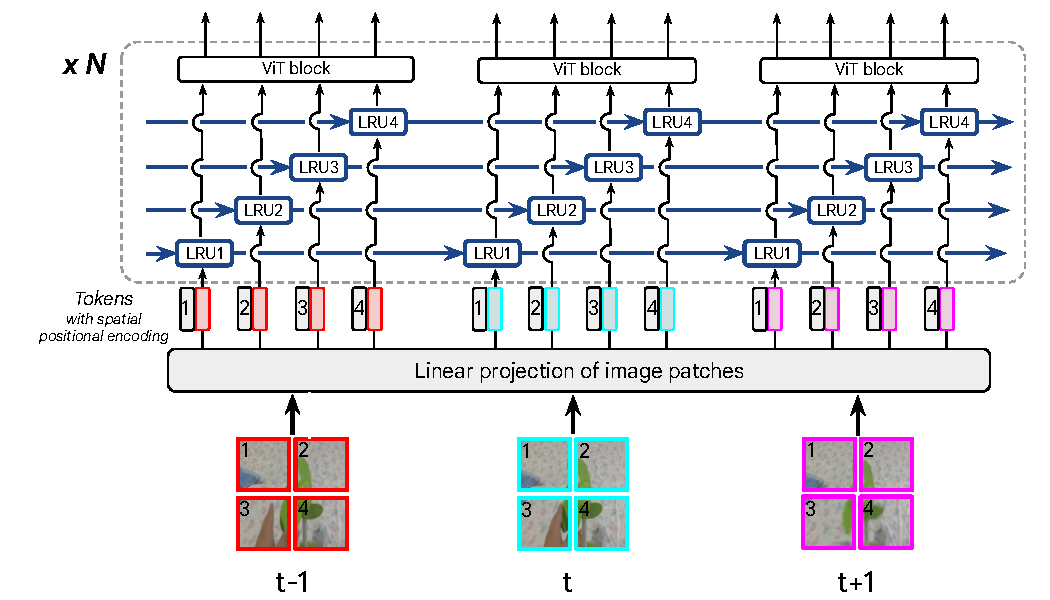
\includegraphics[width=\textwidth]{img/revitmodel.pdf}
%     % \caption{\ssm\ architecture}
% \end{subfigure}%
% \hfill
% \begin{subfigure}{0.34\textwidth}
%     \centering
%     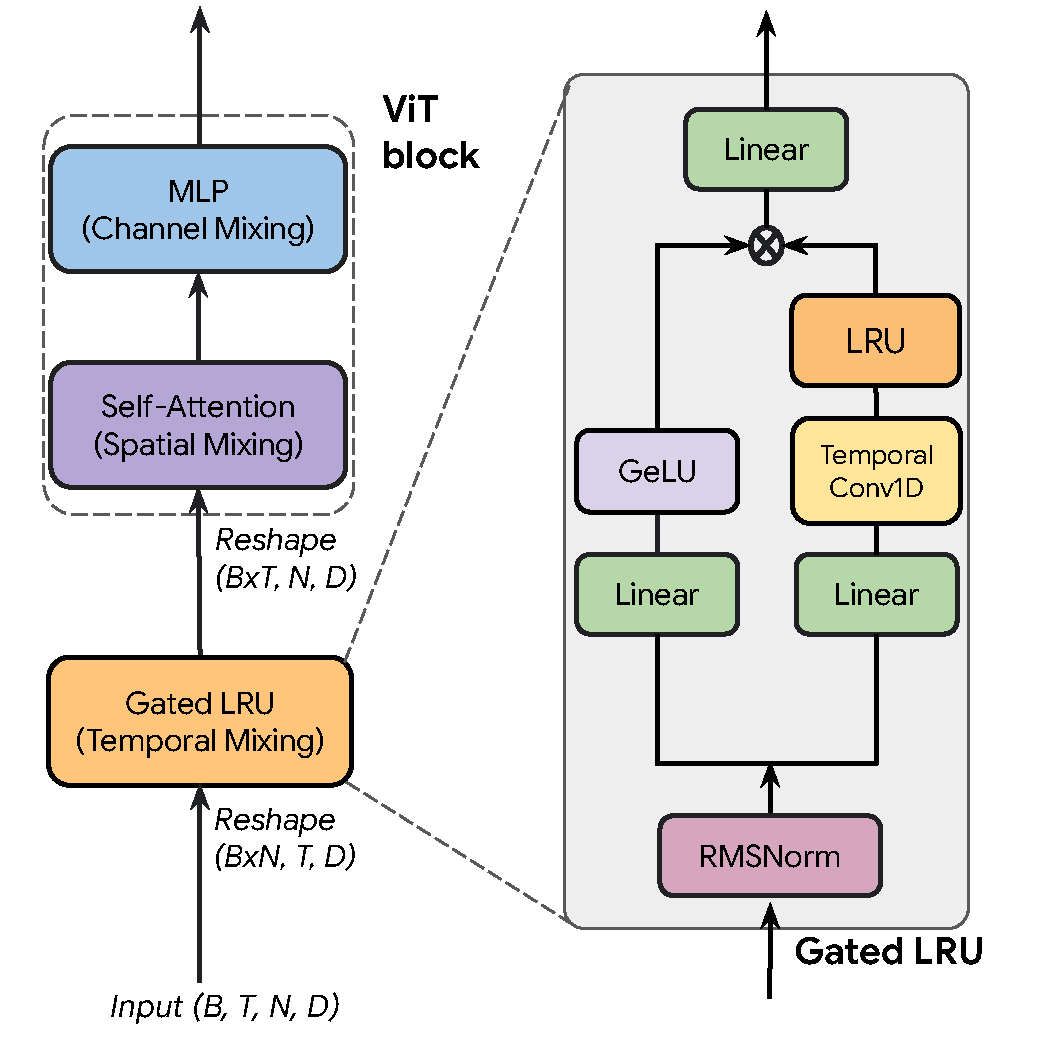
\includegraphics[width=\textwidth]{img/revitblock_tall.pdf} 
%     % \caption{\ssm\ block}
% \end{subfigure}
% % \vspace{-1mm}
% \captionof{figure}{\textbf{Left:} \ssm\ architecture. Each video frame is divided into non-overlapping patches that are linearly projected into a token embedding space. We then add a learnt spatial positional encoding. The tokens are passed through gated linear recurrent units (LRUs) that share parameters across space. The outputs of the recurrent blocks are then processed by a ViT block. The recurrent operation followed by ViT is repeated N times. \textbf{Right:} \ssm\ block. The input is a batch of videos, each frame with N tokens. We apply recurrent units over \textit{temporal tubes} to integrate information over time, and self-attention and MLP across tokens within each frame. Note that the recurrent units share parameters, but the information is not mixed across temporal tubes. Similarly, the ViT blocks share parameters, but the information is not mixed across frames.}
% \vspace{1em}
% \vspace{2mm}
% \label{fig:ssmvit}
% % \end{figure*}
% }]
\twocolumn[{%
\renewcommand\twocolumn[1][]{#1}%
\maketitle
\begin{center} % Center the minipages
\begin{minipage}{0.6\textwidth}
    \centering
    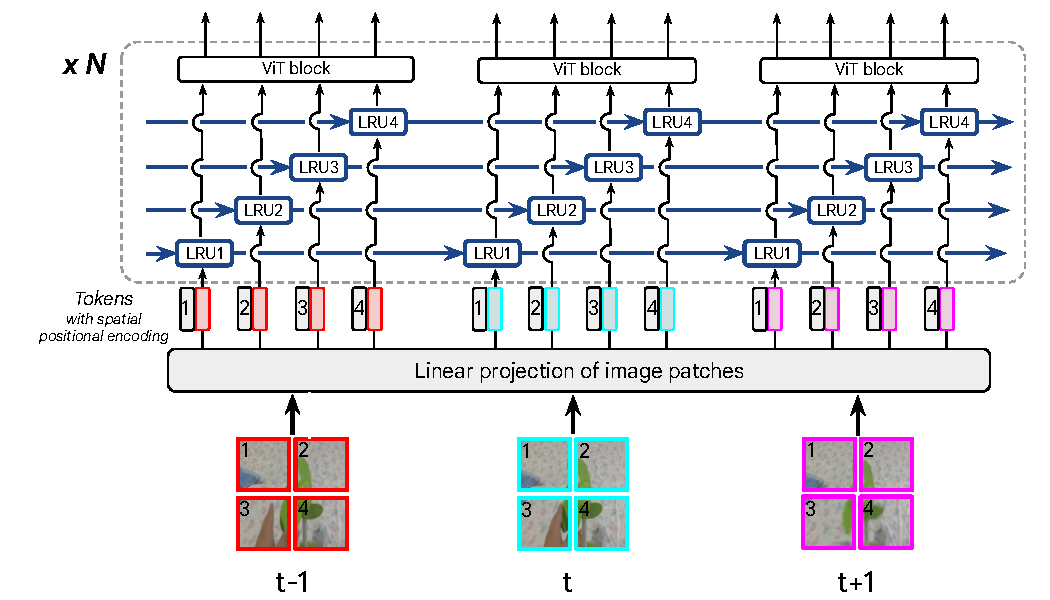
\includegraphics[width=\textwidth]{img/revitmodel.pdf}
\end{minipage}%
\hfill
\begin{minipage}{0.34\textwidth}
    \centering
    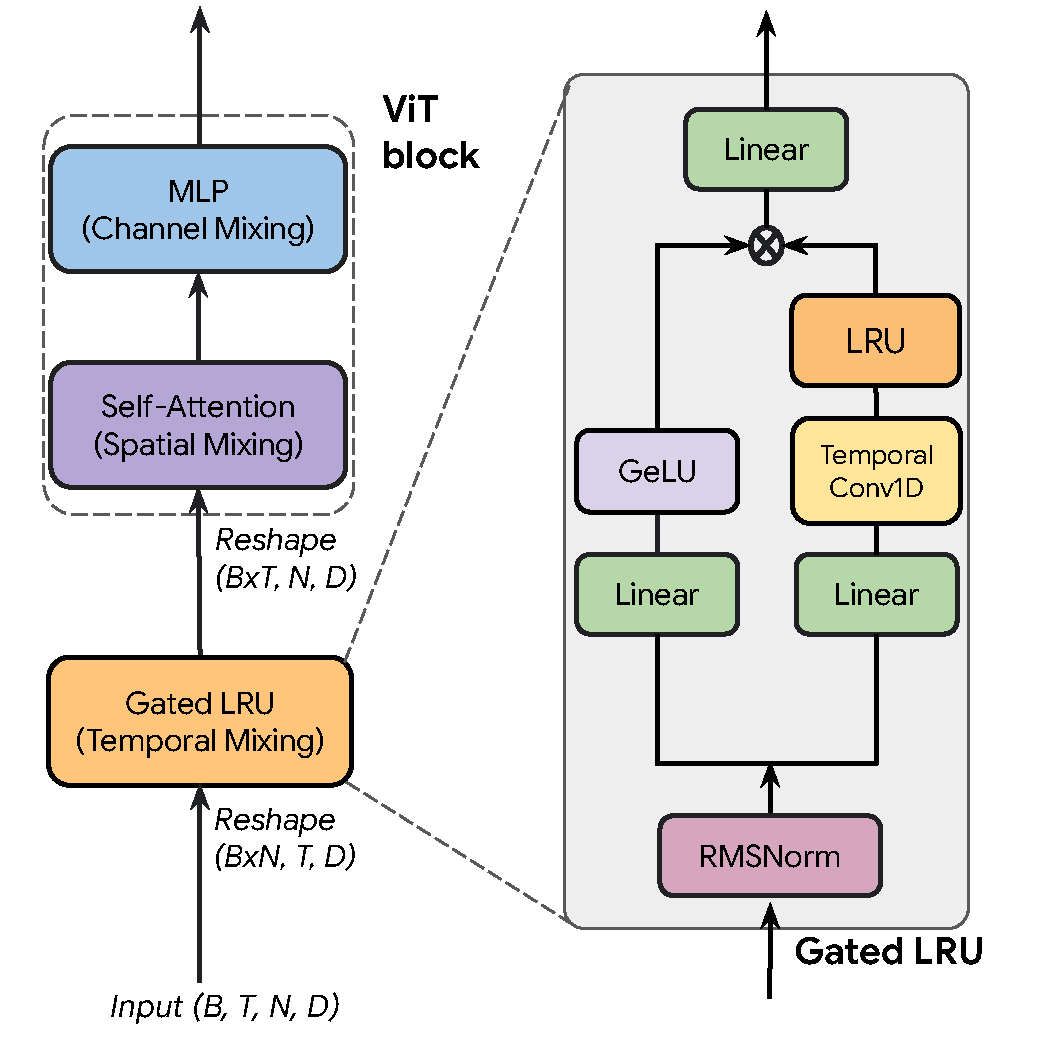
\includegraphics[width=\textwidth]{img/revitblock_tall.pdf}
\end{minipage}
\vspace{-2mm}
\captionof{figure}{\textbf{Left:} \ssm\ architecture. Each video frame is divided into non-overlapping patches that are linearly projected into a token embedding space. We then add a learnt spatial positional encoding. The tokens are passed through gated linear recurrent units (LRUs) that share parameters across space. The outputs of the recurrent blocks are then processed by a ViT block. The recurrent operation followed by ViT is repeated N times. \textbf{Right:} \ssm\ block. The input is a batch of videos, each frame with N tokens. We apply recurrent units over \textit{temporal tubes} to integrate information over time, and self-attention and MLP across tokens within each frame. Note that the recurrent units share parameters, but the information is not mixed across temporal tubes. Similarly, the ViT blocks share parameters, but the information is not mixed across frames.}
% \vspace{1em}
% \vspace{2mm}
\label{fig:ssmvit}
\end{center}

\vspace{1em} 
}] 


\begin{abstract}
Segment Anything Model 2 (SAM 2) has emerged as a powerful tool for video object segmentation and tracking anything. Key components of SAM 2 that drive the impressive video object segmentation performance include a large multistage image encoder for frame feature extraction and a memory mechanism that stores memory contexts from past frames to help current frame segmentation. The high computation complexity of multistage image encoder and memory module has limited its applications in real-world tasks, e.g., video object segmentation on mobile devices. To address this limitation, we propose EfficientTAMs, lightweight track anything models that produce high-quality results with low latency and model size. Our idea is based on revisiting the plain, nonhierarchical Vision Transformer (ViT) as an image encoder for video object segmentation, and introducing an efficient memory module, which reduces the complexity for both frame feature extraction and memory computation for current frame segmentation. We take vanilla lightweight ViTs and efficient memory module to build EfficientTAMs, and train the models on SA-1B and SA-V datasets for video object segmentation and track anything tasks. We evaluate on multiple video segmentation benchmarks including semi-supervised VOS and promptable video segmentation, and find that our proposed EfficientTAM with vanilla ViT perform comparably to SAM 2 model (HieraB+SAM 2) with $\sim$2x speedup on A100 and $\sim$2.4x  parameter reduction. On segment anything image tasks, our EfficientTAMs also perform favorably over original SAM with $\sim$20x  speedup on A100 and $\sim$20x  parameter reduction. On mobile devices such as iPhone 15 Pro Max, our EfficientTAMs can run at $\sim$10 FPS for performing video object segmentation with reasonable quality, highlighting the capability of small models for on-device video object segmentation applications. 
\end{abstract}    
\section{Introduction}
Deep learning techniques have made rapid progress in conditional image generation. For example, networks have been used to inpaint missing image regions~\citep{pathakCVPR16context,yang2016high,isola2016image}, 
add color to grayscale images~\citep{iizuka2016let,larsson2016learning,zhang2016colorful,isola2016image}, and generate photorealistic images from sketches~\cite{sangkloy2017scribbler,isola2016image}.
However, most techniques in this space have focused on generating a \textit{single} result.
In this work, we model a \textit{distribution} of potential results, as many of these problems may be multimodal in nature. For example,
as seen in Figure~\ref{fig:teaser}, an image captured at night may look very different in the day, depending on cloud patterns and lighting conditions.
We pursue two main goals: producing results which are (1) perceptually realistic and (2) diverse, all while remaining faithful to the input.

Mapping from a high-dimensional input to a high-dimensional output distribution is challenging. A common approach to representing multimodality is learning a low-dimensional latent code, which should represent aspects of the possible outputs not contained in the input image. At inference time, a deterministic generator uses the input image, along with stochastically sampled latent codes, to produce randomly sampled outputs. A common problem in existing methods is~\textit{mode collapse}~\citep{goodfellow2016nips}, where only a small number of real samples get represented in the output.
We systematically study a family of solutions to this problem.

We start with the \pp framework~\citep{isola2016image}, which has previously been shown to produce high-quality results for various image-to-image translation tasks. The method trains a generator network, conditioned on the input image, with two losses: (1) a regression loss to produce similar output to the known paired ground truth image and (2) a learned discriminator loss to encourage realism. The authors note that trivially appending a randomly drawn latent code did not produce diverse results. Instead, we propose encouraging a bijection between the output and latent space. 
We not only perform the direct task of mapping the latent code (along with the input) to the output but also jointly learn an encoder from the output back to the latent space. 
This discourages two different latent codes from generating the same output (non-injective mapping).
During training, the learned encoder attempts to pass enough information to the generator to resolve any ambiguities regarding the output mode.
For example, when generating a day image from a night image, the latent vector may encode information about the sky color, lighting effects on the ground, and cloud patterns.  Composing the encoder and generator sequentially should result in the same image being recovered. The opposite should produce the same latent code.

\begin{figure}
\centering
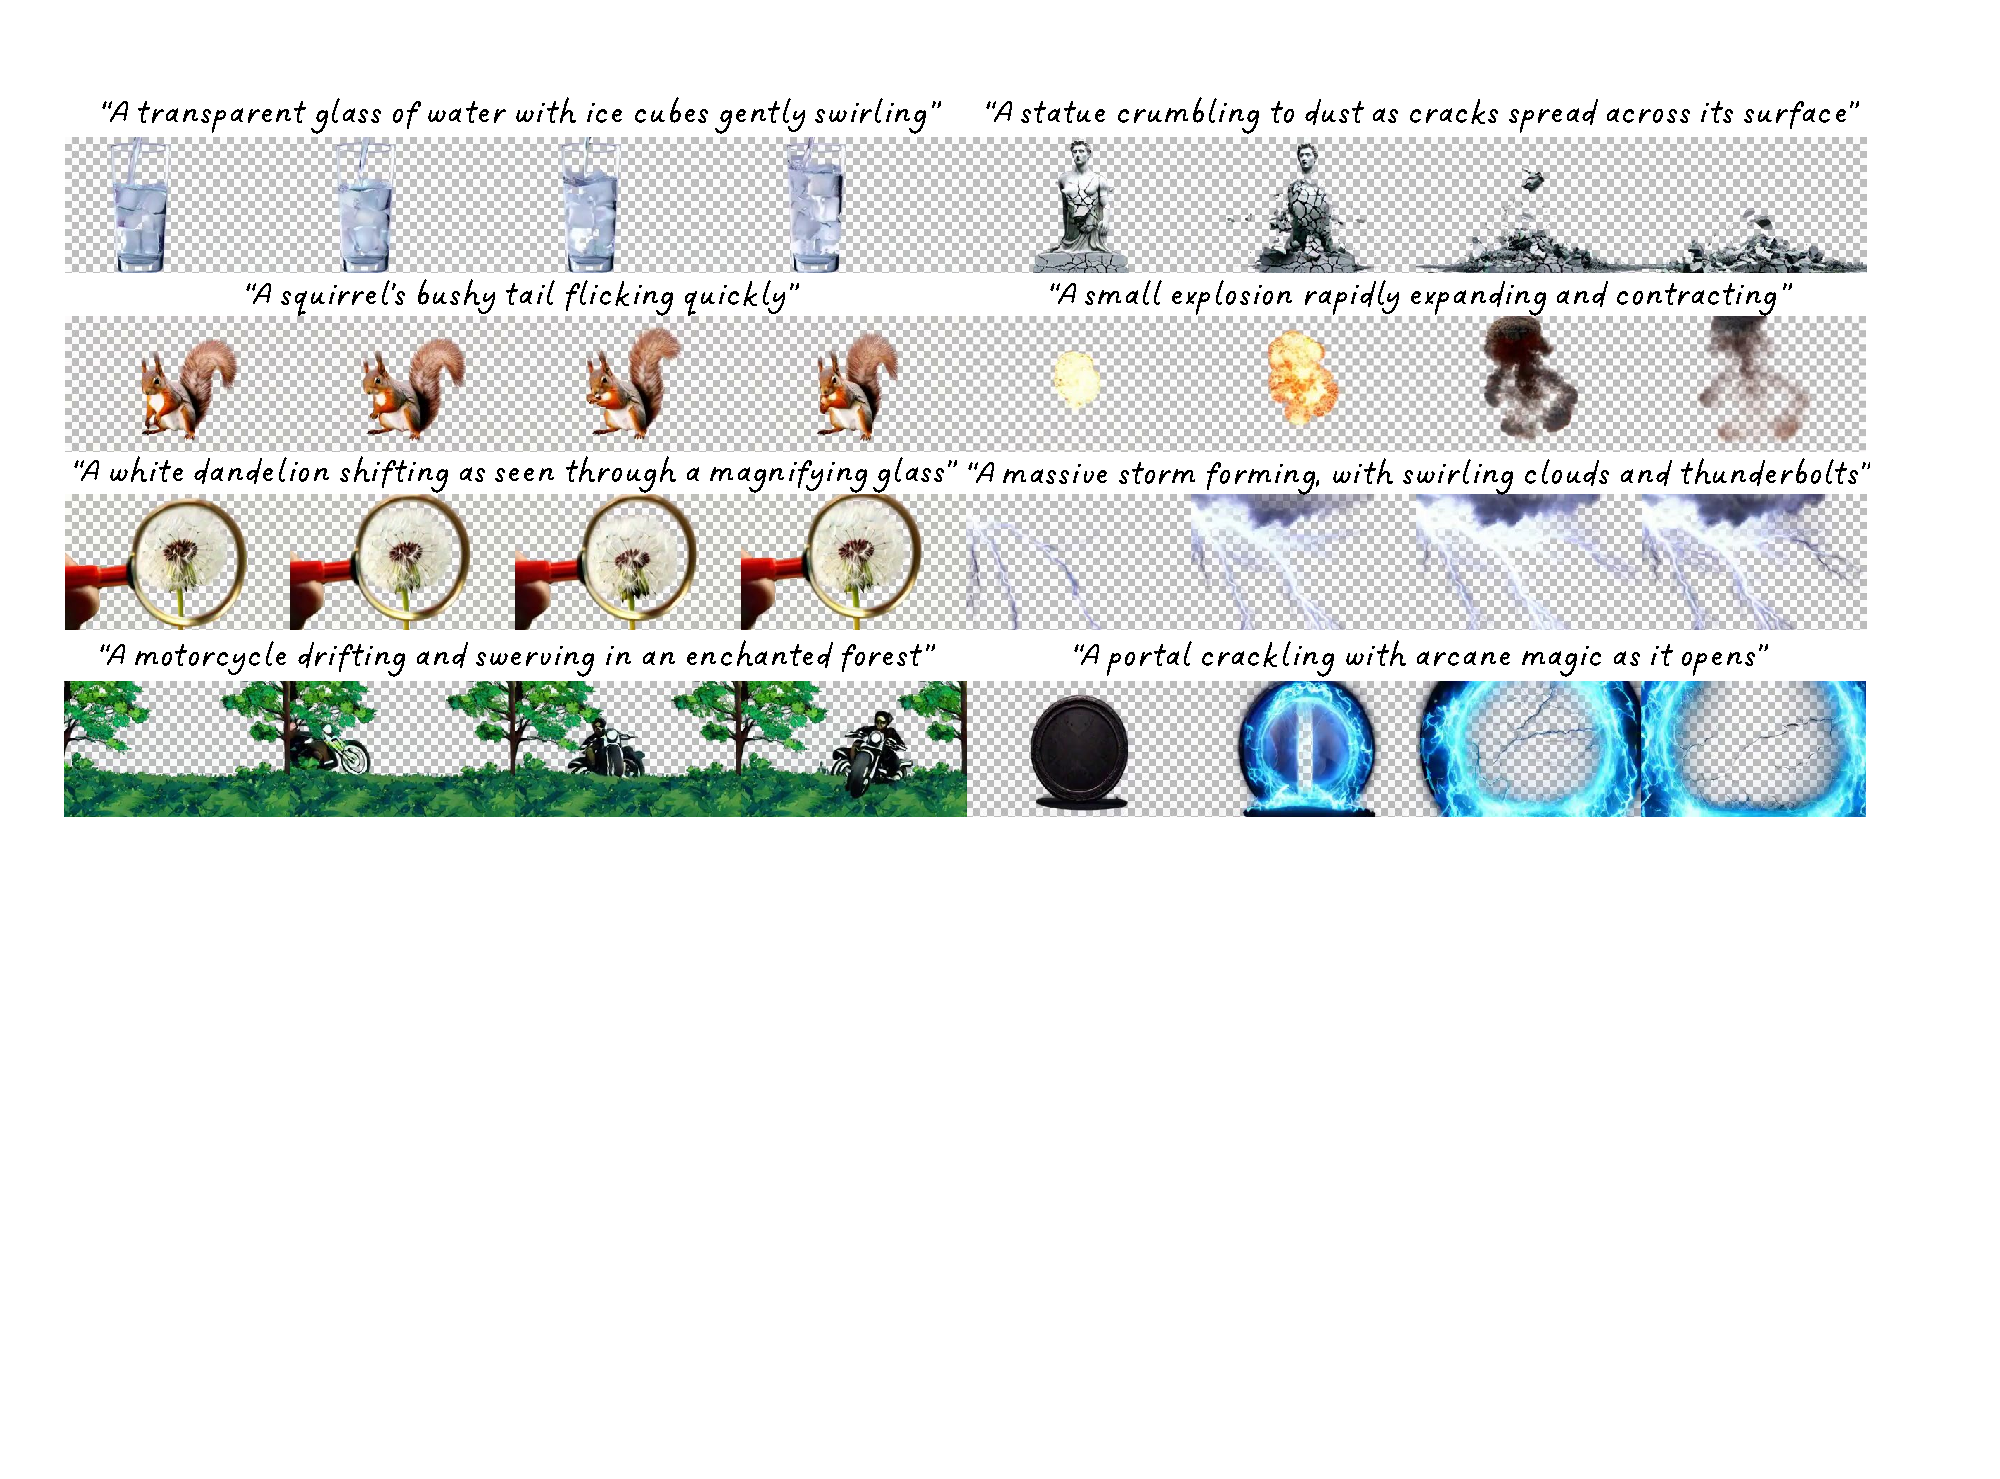
\includegraphics[width=1.\linewidth]{imgs/teaser.pdf}
\vspace{-4mm}
\caption{\small Multimodal image-to-image translation using our proposed method: given an input image from one domain (night image of a scene), we aim to model a \textit{distribution} of potential outputs in the target domain (corresponding day images), producing both realistic and diverse results.}
\vspace{-4mm}
\label{fig:teaser}
\end{figure}


In this work, we instantiate this idea by exploring several objective functions, inspired by literature in unconditional generative modeling:
  \begin{itemize}[leftmargin=0.1in]
  
    \item \textbf{\cvaegan (Conditional Variational Autoencoder GAN)}:
    One approach is first encoding the ground truth image into the latent space, giving the generator a noisy ``peek" into the desired output. Using this, along with the input image, the generator should be able to reconstruct the specific output image. To ensure that random sampling can be used during inference time, the latent distribution is regularized using KL-divergence to be close to a standard normal distribution. This approach has been popularized in the unconditional setting by VAEs~\citep{kingma2013auto} and VAE-GANs~\citep{larsen2016vaegan}.
    
    \item \textbf{\cinfogan (Conditional Latent Regressor GAN)}: Another approach is to first provide a randomly drawn latent vector to the generator. In this case, the produced output may not necessarily look like the ground truth image, but it should look realistic. An encoder then attempts to recover the latent vector from the output image. This method could be seen as a conditional formulation of the ``latent regressor" model~\citep{donahue2016adversarial,dumoulin2016adversarially} and also related to InfoGAN~\citep{xi2016infogan}.
    
    \item \textbf{\bicycle}: Finally, we combine both these approaches to enforce the connection between latent encoding and output in both directions {\em jointly} and achieve improved performance. We show that our method can produce both diverse and visually appealing results across a wide range of image-to-image translation problems, significantly more diverse than other baselines, including naively adding noise in the \pp framework. In addition to the loss function, we study the performance with respect to several encoder networks, as well as different ways of injecting the latent code into the generator network. 
\end{itemize}

We perform a systematic evaluation of these variants by using humans to judge photorealism and a perceptual distance metric~\cite{zhang2018unreasonable} to assess output diversity. Code and data are available at \url{https://github.com/junyanz/BicycleGAN}.
\section{Related Work}
\label{sec:related work}

\begin{figure*}[t]
    \centering
    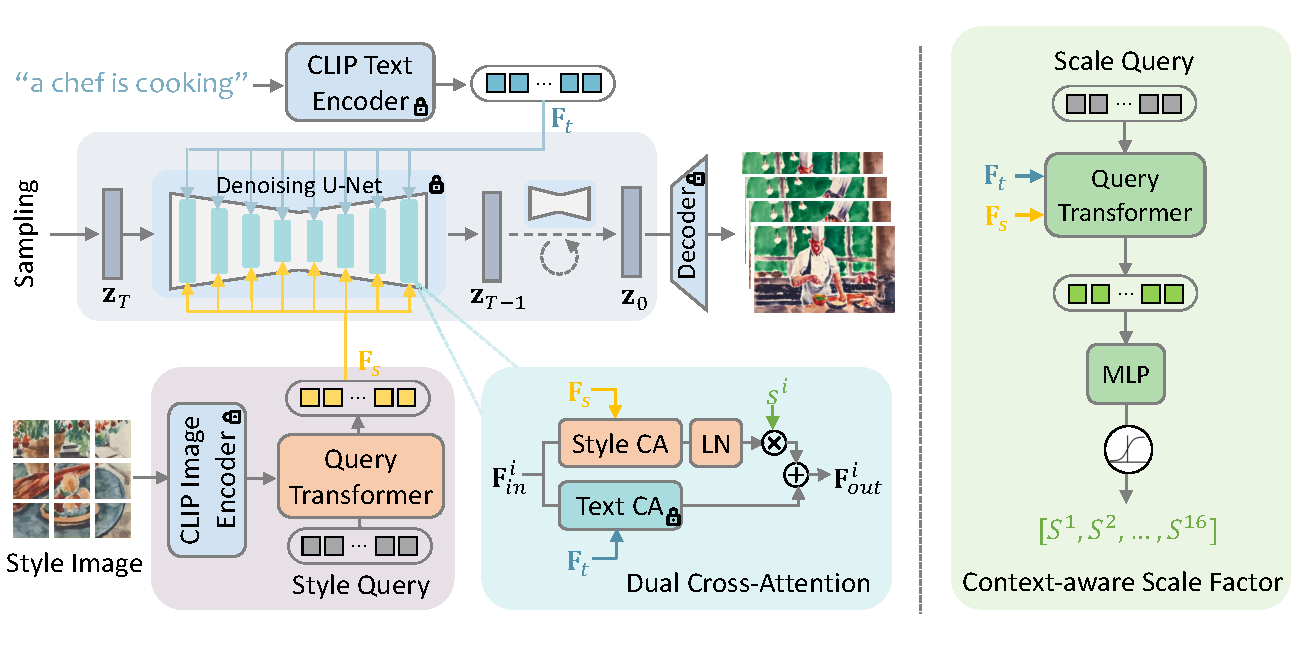
\includegraphics[width=1\linewidth]{figure/overview.pdf}\vspace{-2mm}
    \caption{Overview of the proposed~\name.}
    \label{fig:overview}
\end{figure*}

% \textbf{Video Super-Resolution.}
\paragraph{Video Super-Resolution.} 
Traditional VSR methods can be roughly divided into two categories: recurrent-based \cite{haris2019recurrent, huang2017video, liang2022recurrent, sajjadi2018frame, shi2022rethinking} and sliding-window-based \cite{caballero2017real,liang2024vrt,li2020mucan,xu2021temporal,yi2019progressive} methods. 
Recurrent-based methods process LR video frame by frame using recurrent neural networks \cite{mikolov2010recurrent}. In contrast, sliding-window-based methods divide a video sequence into segments, using each as input to super-resolve the video. 
However, both approaches suffer from degradation mismatch, leading to significant performance drops in real-world applications.
Recently, there has been a growing focus on real-world VSR, targeting complex, unknown degradations. RealBasicVSR \cite{chan2022investigating}, an extension of BasicVSR \cite{chan2021basicvsr}, introduces a pre-cleaning module to mitigate artifacts. 
RealViformer \cite{zhang2024realviformer} discovers that channel attention is less sensitive to artifacts and uses squeeze-excite mechanisms and covariance-based rescaling to address these challenges further. While GAN-based and image diffusion models have made substantial progress, they still face issues such as \textit{over-smoothing details and temporal inconsistency}.

\vspace{-1em}
\paragraph{Text-to-Video Diffusion Model.} 
% \noindent
% \textbf{Text-to-Video Diffusion Model.}
Large-scale pre-trained text-to-video (T2V) diffusion models have garnered significant attention, particularly with the impressive results from Sora \cite{videoworldsimulators2024,sora}. 
Numerous T2V models have since emerged, generally divided into: U-Net-based methods \cite{blattmann2023align, blattmann2023stable, ho2022imagen, singer2022make} and DiT-based methods \cite{yang2024cogvideox, bao2024vidu, polyak2024movie, chen2024gentron}. 
I2VGen-XL \cite{zhang2023i2vgen}, a U-Net-based method, employs a two-stage approach: first generating semantically and content-consistent LR videos, then using these as conditions to produce HR outputs.
CogvideoX \cite{yang2024cogvideox}, built on DiT \cite{peebles2023scalable}, introduces an adaptive LayerNorm to enhance text-video alignment and employs 3D attention to better integrate spatio-temporal information.
Both models %, regardless of architecture, 
have large model capacities and are trained on large-scale datasets, enabling them to capture robust spatio-temporal priors. 
In this work, we propose~\name~to \textit{fully leverage T2V model prior for real-world VSR}.

\vspace{-1em}
\paragraph{Diffusion Prior for Super-Resolution.}
% \noindent
% \textbf{Diffusion Prior for Super-Resolution.}
Several works \cite{wang2024exploiting, lin2023diffbir, yang2023pixel, wu2024seesr, zhao2024wavelet} have leveraged generative diffusion priors for image and video super-resolution. 
StableSR \cite{wang2024exploiting} adds a time-aware encoder and feature warping module to the SD model. DiffBIR \cite{lin2023diffbir} integrates restoration and generative modules via ControlNet, while PASD \cite{yang2023pixel} and SeeSR \cite{wu2024seesr} embed semantic information in U-Net to guide diffusion. These methods balance fidelity and perceptual quality, achieving high-resolution image details.
Methods like Upscale-A-Video \cite{zhou2024upscale}, MGLD-VSR \cite{yang2023mgldvsr}, Inflating with Diffusion \cite{yuan2024inflation}, and SATeCo \cite{chen2024learning} have adapted text-to-image diffusion priors~\cite{rombach2022high,ho2022imagen} for VSR by adding temporal layers. However, rooted in text-to-image models, they often struggle with temporal consistency. 
More recently, VEnhancer\cite{he2024venhancer} and LaVie-SR\cite{wang2023lavie} have incorporated T2V models to super-resolve AI-generated videos but struggle with complex degradations in practical environments. 
In contrast, we are the \textit{first} to integrate powerful T2V diffusion priors for real-world VSR, introducing the LIEM module to address spatial artifacts and DF loss to enhance fidelity.
\section{Method}
\label{sec:method}

\begin{figure*}[t]
    \centering
    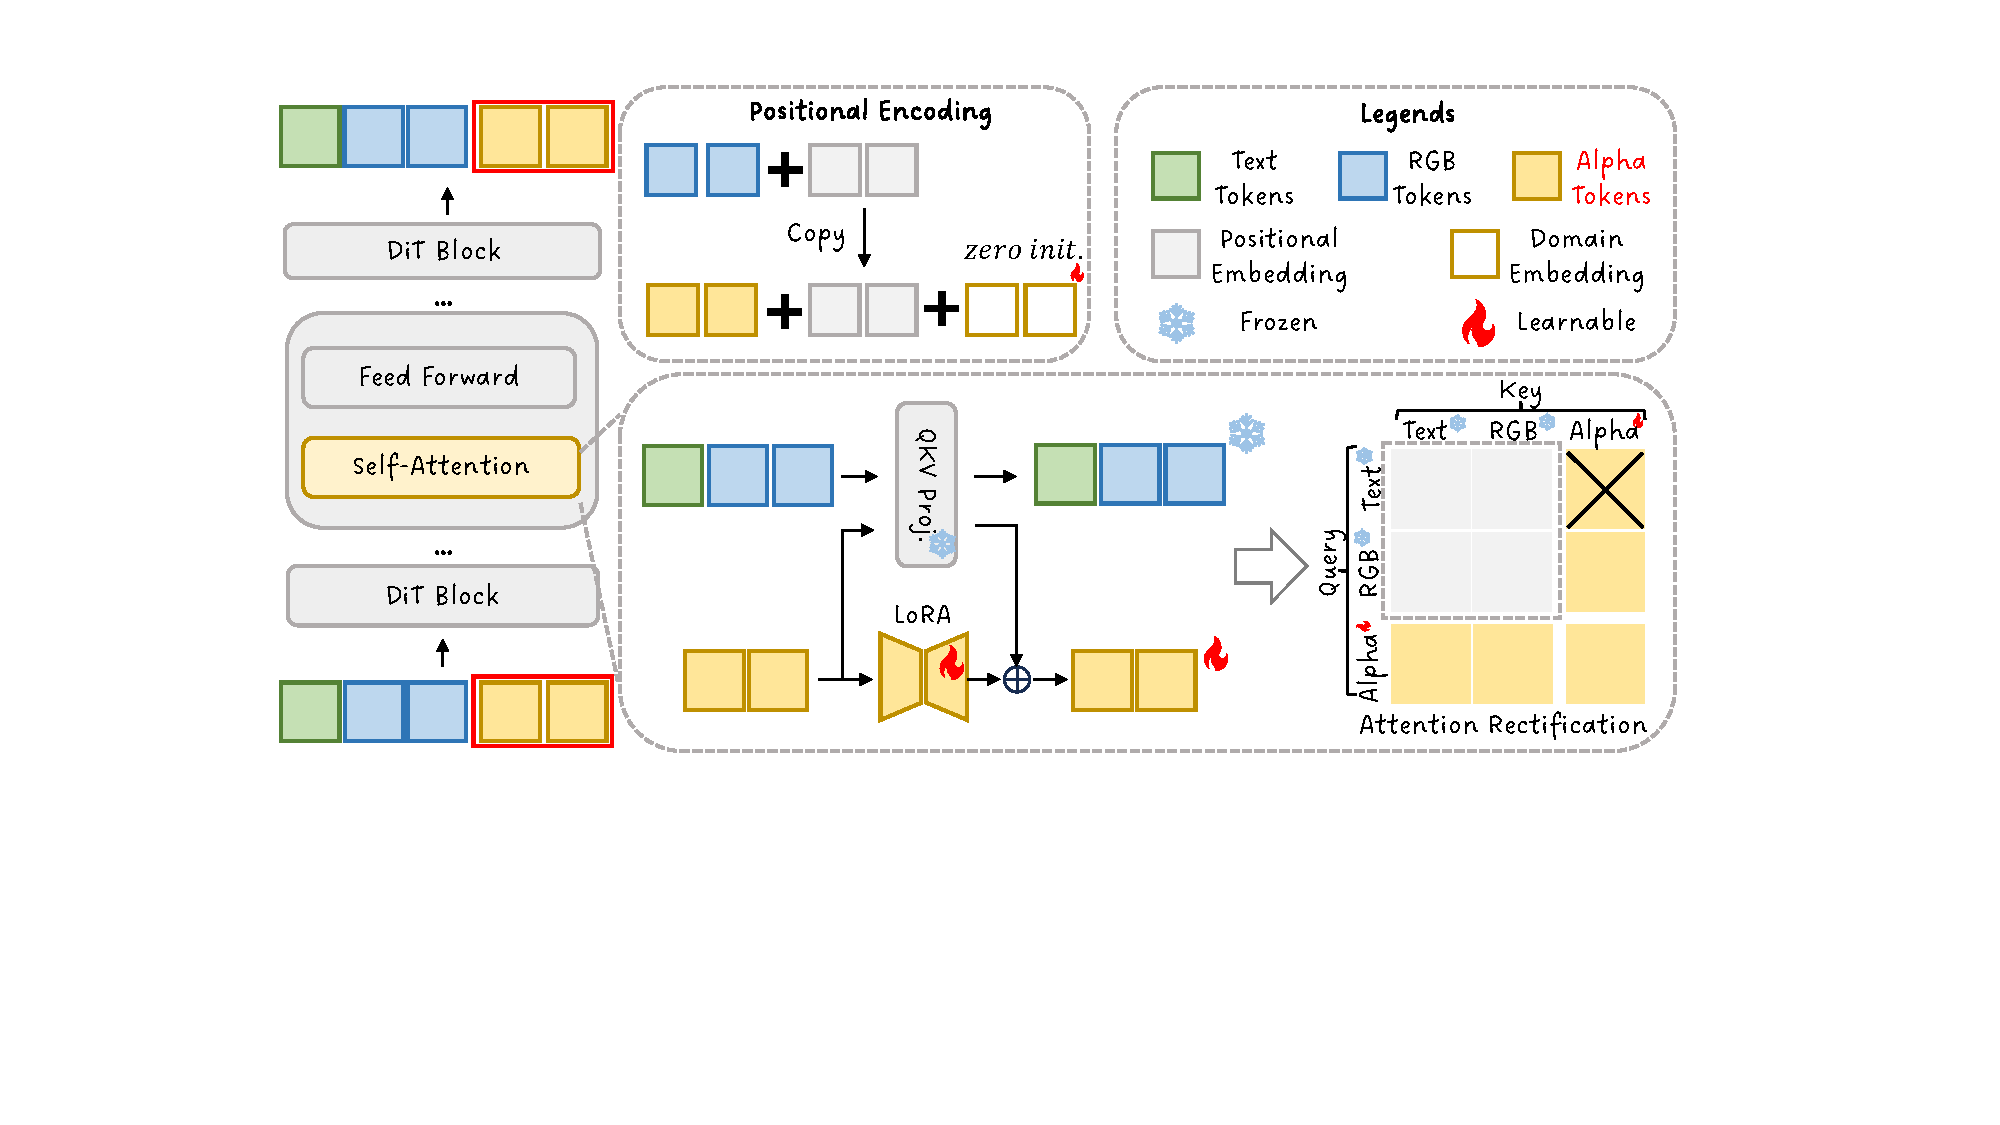
\includegraphics[width=1.0\linewidth]{figs/method-pipeline.pdf}
    \vspace{-0.2in}
    \caption{\textbf{Pipeline of TransPixar.} Our method is organized as follows: (1) \textbf{Left}: we extend the input of DiT to include new alpha tokens; (2) \textbf{Top Center}: we initialize alpha tokens with our positional encoding; (3) \textbf{Bottom Cente}r: we insert a partial LoRA and adjust attention computation during training and inference.}
    \label{fig-pipeline}
    \vspace{-0.1in}
\end{figure*}


% %-------------------------------------------------------------------------
\subsection{Preliminary}
We first introduce the open-sourced state-of-the-art DiT-based video generation models~\cite{yang2024cogvideox,genmo2024mochi}.
The core components of DiT-based video models are attention modules, and there are two primary distinctions between these models and previous approaches.
On one hand, unlike previous models that alternate between 1D temporal attention and 2D spatial attention~\cite{cerspense2023zeroscope, chen2023videocrafter1, chen2024videocrafter2, opensora}, current methods typically employ 3D spatio-temporal attention, allowing them to capture spatio-temporal dependencies more effectively.
On the other hand, instead of using cross-attention for text conditioning, these models concatenate text tokens \( \mathbf{x}_{\text{text}} \) with visual tokens \( \mathbf{x}_{\text{video}} \) into a single long sequence. 
The shape of video tokens and text tokens are \(B\times L\times D\) and \(B\times L_{\text{text}}\times D\), wher \(B\) equals to batch size, \(L_{\text{text}}\) equals to the length of text tokens, \(L\) equals to the length of video tokens and \(D\) equals to the latent dimension of transformer.
Full self-attention is then applied across the combined sequence:
\begin{equation}
\begin{aligned}
    &\text{Attention}(\mathbf{Q}, \mathbf{K}, \mathbf{V}) = \text{softmax}\left(\frac{\mathbf{Q}\mathbf{K}^T}{\sqrt{d_k}}\right)\mathbf{V}, \quad \text{where} \\
&\mathbf{Z : Z \in \{Q, K, V\}} \\&= [\mathbf{W}_{z : z \in \{q, k, v\}}(\mathbf{x}_{\text{text}}); \mathbf{f}_{z : z \in \{q, k, v\}}(\mathbf{x}_{\text{video}})]
\end{aligned}
\label{SA}
\end{equation}


Here \( \mathbf{W}_{t} \) (for \( t \in \{q, k, v\} \)) represents the projection matrixs in the transformer model, and \( \mathbf{f}_{t} \) (for \( t \in \{q, k, v\} \)) represents a combined operation that incorporates both the projection and positional encoding for visual tokens. 
There are two commonly used types of positional encoding. One is absolute positional encoding formulated as follows:
\begin{equation}
\begin{aligned}
\mathbf{f}_{z : z \in \{q, k, v\}}(\mathbf{x}_{\text{video}}) := \mathbf{W}_{z : z \in \{q, k, v\}}(\mathbf{x}_{\text{video}}^m + \mathbf{p}^m),
\end{aligned}
\label{PE}
\end{equation}
where \( \mathbf{p} \) is the positional embedding (e.g., a sinusoidal function) and \( m \) denotes the position of each RGB video token.
Another approach is the Rotary Position Embedding (RoPE)~\cite{su2024roformer}, often used by~\cite{yang2024cogvideox, genmo2024mochi}. 
This is expressed as
\begin{equation}
\begin{aligned}
\mathbf{f}_{z : z \in \{q, k\}}(\mathbf{x}_{\text{video}}) := \mathbf{W}_{z : z \in \{q, k\}}(\mathbf{x}_{\text{video}}^m) \circ e^{im\theta},
\end{aligned}
\label{RoPE}
\end{equation}
where \( m \) is the positional index, \( i \) is the imaginary unit for rotation, and \( \theta \) is the rotation angle.




% %-------------------------------------------------------------------------
\subsection{Our Approach} 
To jointly generate RGB and alpha videos, we adapt a pretrained RGB video generation model through several modifications. The whole pipeline is visualized in Fig.~\ref{fig-pipeline}.

Firstly, we double the sequence length of noisy input tokens to enable the model to generate videos of double length, from \( \mathbf{x}^{1:L}_{\text{video}} \) to \( \mathbf{x}^{1:2*L}_{\text{video}} \). 
Here, \( \mathbf{x}^{1:L}_{\text{video}} \) will be decoded into the RGB video, while \( \mathbf{x}^{L+1:2*L}_{\text{video}} \) will be decoded into the corresponding alpha video.
The Query(Q), Key(K), Value(V) representations are formulated as:
\begin{equation}
\begin{aligned}
&\mathbf{Z : Z \in \{Q, K, V\}} \\&= [\mathbf{W}_{z : z \in \{q, k, v\}}(\mathbf{x}_{\text{text}}); \mathbf{f}_{z : z \in \{q, k, v\}}(\mathbf{x}^{1:2*L}_{\text{video}})]
\end{aligned}
\end{equation}

In addition to sequence doubling, we explored increasing batch size or latent dimensions and splitting output into two domains; however, these approaches showed limited effectiveness under constrained datasets, which we discuss later.

Secondly, we modify the positional encoding function \( \mathbf{f}_{t : t \in \{q, k, v\}}(\cdot) \), as shown in Fig.~\ref{fig-pe}.
Instead of continuously numbering indices, we allow RGB and alpha tokens to share the same positional encoding. 
Taking absolute positional encoding as an example:
\begin{equation}
\begin{aligned}
&\mathbf{f}^*_{z : z \in \{q, k, v\}}(\mathbf{x}_{\text{video}}) \\:=
&\begin{cases}
\mathbf{W}_{z : z \in \{q, k, v\}}(\mathbf{x}_{\text{video}}^m + \mathbf{p}^m), & \text{if } m \leq L, \\
\mathbf{W}^*_{z : z \in \{q, k, v\}}(\mathbf{x}_{\text{video}}^m + \mathbf{p}^{m-L} + d), & \text{if } m > L.
\end{cases}
\label{eq:our_pe}
\end{aligned}
\end{equation}

Here we introduce a domain embedding \( d \), initialized to zero. We make it learnable to help the model adaptively differentiate between RGB (\(m\leq L\)) and alpha tokens (\(m>L \)). 
%
The motivation behind this design is we observe that with same postional encoding, even initializing with different noises, the tokens from two domains tend to generate same results. 
It minimizes spatial-temporal alignment challenges at the very beginning of training and thus accelerates convergence.

Next we propose a fine-tuning scheme using LoRA~\cite{hu2021lora}, in which the LoRA layer is applied only to alpha domain tokens:
\begin{equation}
\begin{aligned}
&\mathbf{W}^*_{z : z \in \{q, k, v\}}(\mathbf{x}_{\text{video}}^m + \mathbf{p}^{m-L} + d)\\=
&\ \mathbf{W}_{z : z \in \{q, k, v\}}(\mathbf{x}_{\text{video}}^m + \mathbf{p}^{m-L} + d)
\\
+\ &\gamma\cdot \text{LoRA}(\mathbf{x}_{\text{video}}^m + \mathbf{p}^{m-L} + d), \quad \text{if } m > L,
\label{eq:our_lora}
\end{aligned}
\end{equation}
where \( \gamma \) controls the residual strength. 
Additionally, we design an attention mask to block unwanted attention computation. 
Given a text-video token sequence length \( L_\text{text} + 2L \), where \( L_\text{text} \) represents text token length, the mask is defined as:
\begin{equation}
\mathbf{M}^*_{mn} = 
\begin{cases} 
-\infty, & \text{if } m \leq L_\text{text} \ \text{and} \ \, n > L_\text{text} + L, \\
0, & \text{otherwise}.
\end{cases}
\label{eq:attn_mask}
\end{equation}

Combining these modifications, inference with our method is expressed as:
\begin{equation}
\begin{aligned}
    &\text{Attention}(\mathbf{Q}, \mathbf{K}, \mathbf{V}) = \text{softmax}\left(\frac{\mathbf{Q}\mathbf{K}^T}{\sqrt{d_k}}+\mathbf{M}^*\right)\mathbf{V}, \quad \text{where} \\
&\mathbf{Z : Z \in \{Q, K, V\}} \\&= [\mathbf{W}_{z : z \in \{q, k, v\}}(\mathbf{x}_{\text{text}}); \mathbf{f}^*_{z : z \in \{q, k, v\}}(\mathbf{x}_{\text{video}})]
\end{aligned}
\label{eq:our_method}
\end{equation}

Training is carried out using flow matching~\cite{liu2022flow} or a traditional diffusion process~\cite{ho2020denoising}.


\begin{figure}[t]
    \centering
    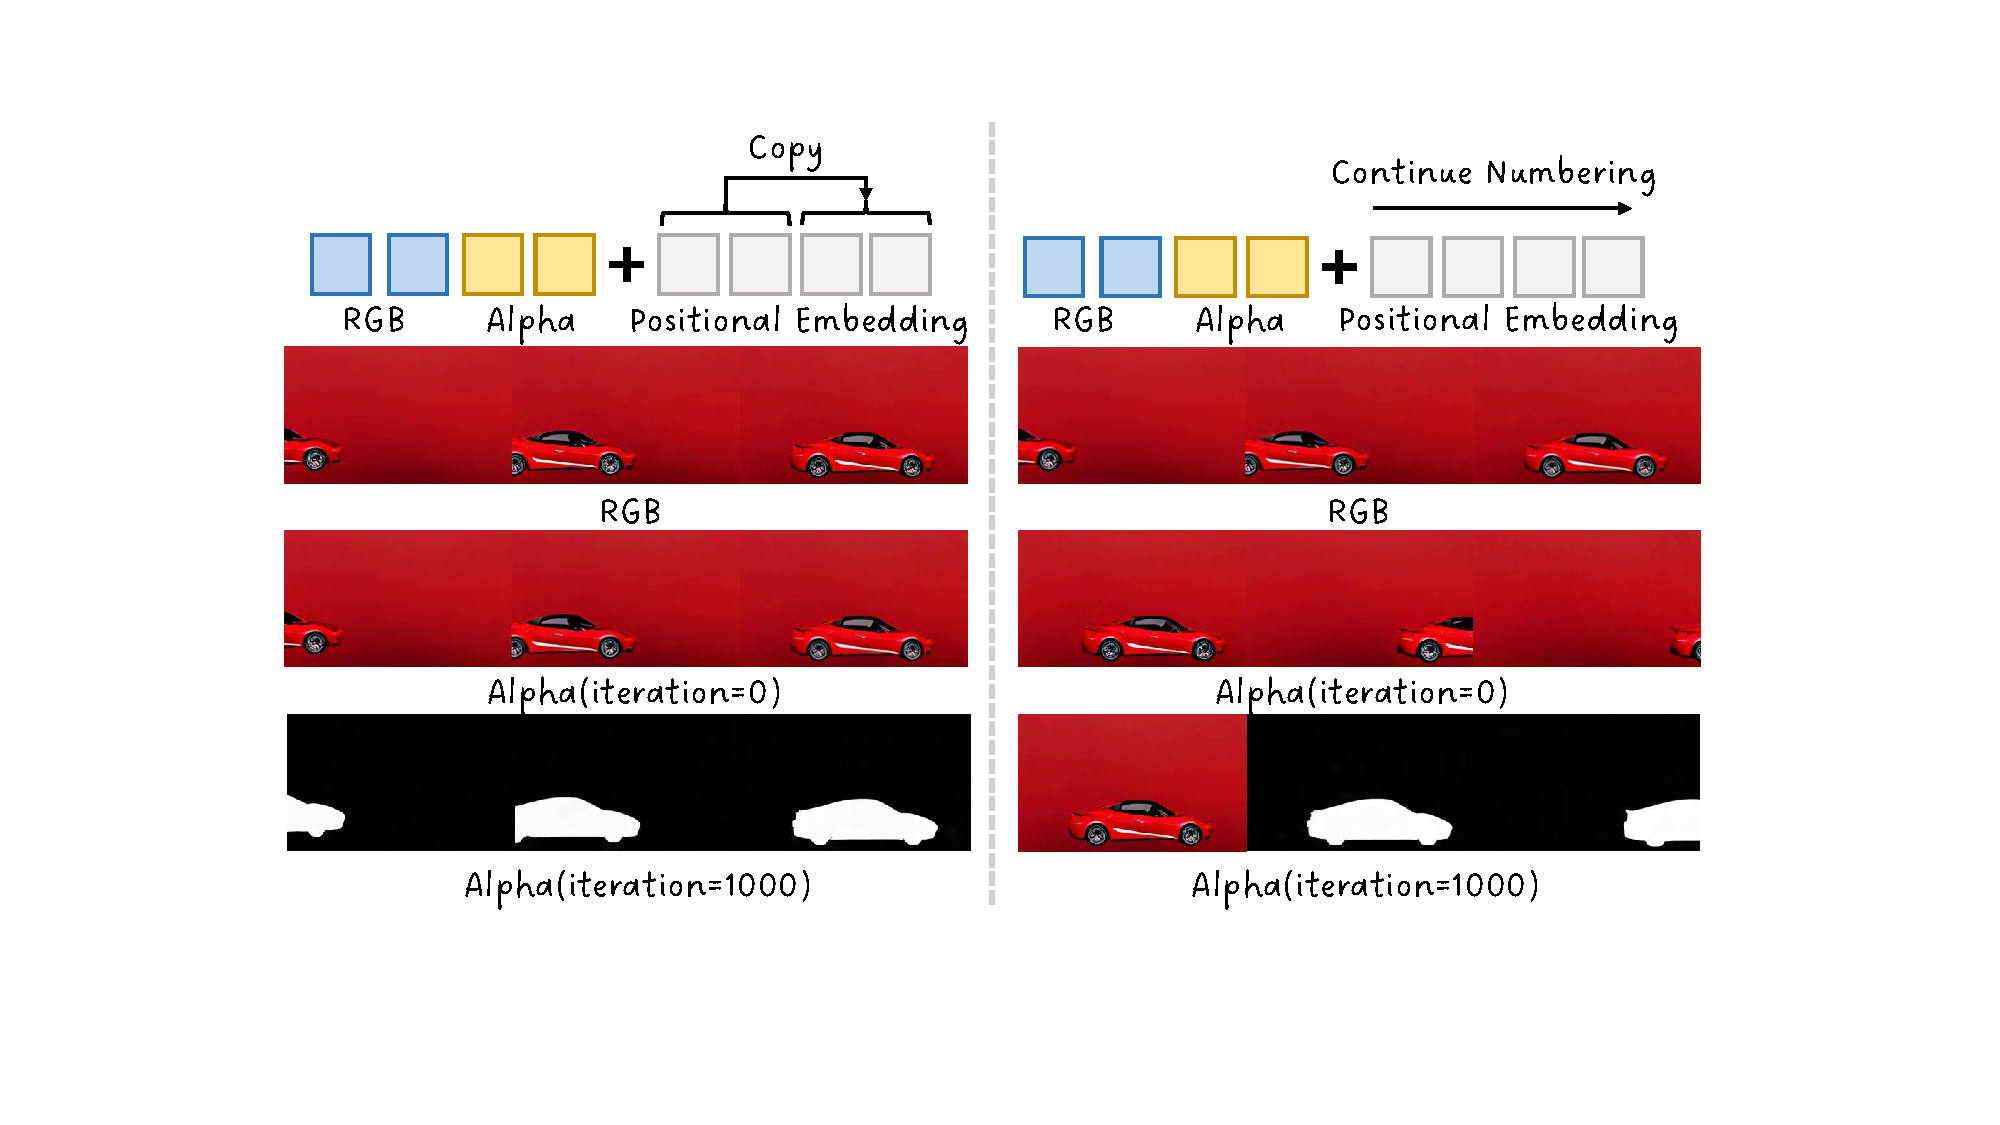
\includegraphics[width=1.0\linewidth]{figs/method-pe_init.pdf}
    \vspace{-0.2in}
    \caption{\textbf{Positional Encoding Design for RGBA Generation.} Assigning alpha tokens the same positional encoding as RGB yields similar results, resulting in faster convergence after 1000 iterations compared to standard encoding strategies.}
    \label{fig-pe}
    \vspace{-0.1in}
\end{figure}

% %-------------------------------------------------------------------------
\subsection{Analysis}
% % given our goal is 最大程度地继承 pretrain video model的能力,让它能生成的东西超越已有的RGBA训练集,
% 在目前我们使用的3d full attention DiT的video generation model的框架下,最重要的计算是attention mechanism,因此我们进一步对该过程进行分析:
% The attention matrix, \(\mathbf{Q}\mathbf{K}^T\), now has dimensions \((L_\text{text} + 2*L) \times (L_\text{text} + 2*L)\), which we simplify by organizing it into a 3x3 grouped attention matrix—\textbf{Text-attend-to-RGB}, \textbf{RGB-attend-to-Text}, and so forth, as illustrated in Fig.~\ref{fig-pipeline}. Then we procceed to analyze them:

% \noindent{\textbf{Text-Attend-to-RGB} and \textbf{RGB-Attend-to-Text}}.
% Given this matrix, we are supposed to preserve as much of the computation in the upper-left 2x2 section as possible so that we can preserve the RGB generation potential. 

% These represent the upper-left 2x2 section in \(\mathbf{Q}\mathbf{K}^T\) and 是RGB original generation model有且仅有的计算过程,如果我们能保证这部分计算不受影响,we can replicate the original RGB generation performance. 
% Therefore, we limited the scope of LoRA's influence, as defined in Equation~\eqref{eq:our_lora}, we retain the original QKV values for both text and RGB tokens, maintaining the pretrained model’s behavior in these domains.

% Besides the partial lora, the introduction of alpha tokens make the text and RGB tokens need to act as key and interact with alpha tokens as query, which will also 改变这个2x2 attention matrix的计算结果。
% Therefore, we proceed to analyze two additional attention computations that affect RGB generation shown in Fig.~\ref{fig-attn}:


% \noindent{\textbf{Text-Attend-to-Alpha}}: We find this attention is detrimental to the generation quality. 
% Since the model is originally trained with text and RGB data, introducing attention from text to alpha causes interference due to the domain gap between alpha and RGB. 
% Specifically, alpha modality provide only contour information and lack the rich texture, color, and semantic details associated with text prompt, thereby degrading generation quality. 
% To mitigate this, we design the attention mask (Equation~\eqref{eq:attn_mask}) that blocks this computation.

% \noindent{\textbf{RGB-Attend-to-Alpha}}: In contrast, we identify \textbf{RGB-to-Alpha} as essential for successful joint generation. 
% This attention allows the model to refine RGB tokens by considering alpha information, facilitating alignment between generated RGB and alpha channels. 
% This refinement process is a critical component missing in prior generation-then-prediction pipelines, which lack a feedback mechanism for RGB refinement based on alpha guidance.
Given our goal of maximizing the inherited capabilities of the pretrained video model, enabling it to generate beyond the existing RGBA training set, we analyze the most critical component within our current 3D full attention DiT video generation model: the attention mechanism.
%
The attention matrix, \(\mathbf{Q}\mathbf{K}^T\), has dimensions \((L_\text{text} + 2*L) \times (L_\text{text} + 2*L)\), which we simplify by organizing it into a 3x3 grouped attention matrix—including \textbf{Text-attend-to-RGB}, \textbf{RGB-attend-to-Text}, and so forth, as illustrated in Fig.~\ref{fig-pipeline}. %We then analyze these components:

\vspace{0.5em}
\noindent\textbf{Text-Attend-to-RGB and RGB-Attend-to-Text}. These represent the upper-left 2x2 section of  and are computations that exist solely in the original RGB generation model. If we ensure that this part of the computation remains unaffected, we can replicate the original RGB generation performance. Therefore, we limit the scope of LoRA's influence, as defined in Eq.~\eqref{eq:attn_mask}, by retaining the original QKV values for both text and RGB tokens, thus preserving the pretrained model’s behavior in these domains.

Besides the partial LoRA, the added alpha tokens requires the text and RGB tokens to also act as queries and interact with the alpha tokens as keys, which alters the computation in this 2x2 attention matrix. 
Therefore, we further analyze two additional attention computations that impact RGB generation, as shown in Fig.~\ref{fig-attn}.

\vspace{0.5em}
\noindent\textbf{Text-Attend-to-Alpha.} We find that this attention is detrimental to the generation quality. Since the model was originally trained with text and RGB data, introducing attention from text to alpha causes interference due to the domain gap between alpha and RGB. Specifically, the alpha modality provides only contour information and lacks the rich texture, color, and semantic details associated with the text prompt, thereby degrading generation quality. To mitigate this, we design the attention mask (Eq.~\eqref{eq:attn_mask}) that blocks this computation.

\vspace{0.5em}
\noindent\textbf{RGB-Attend-to-Alpha.} In contrast, we identify \textbf{RGB-to-Alpha} as essential for successful joint generation. This attention allows the model to refine RGB tokens by considering alpha information, facilitating alignment between generated RGB and alpha channels. This refinement process is a critical component missing in previous generation-then-prediction pipelines, which lacked a feedback mechanism for RGB refinement based on alpha guidance.


\begin{figure}[t]
    \centering
    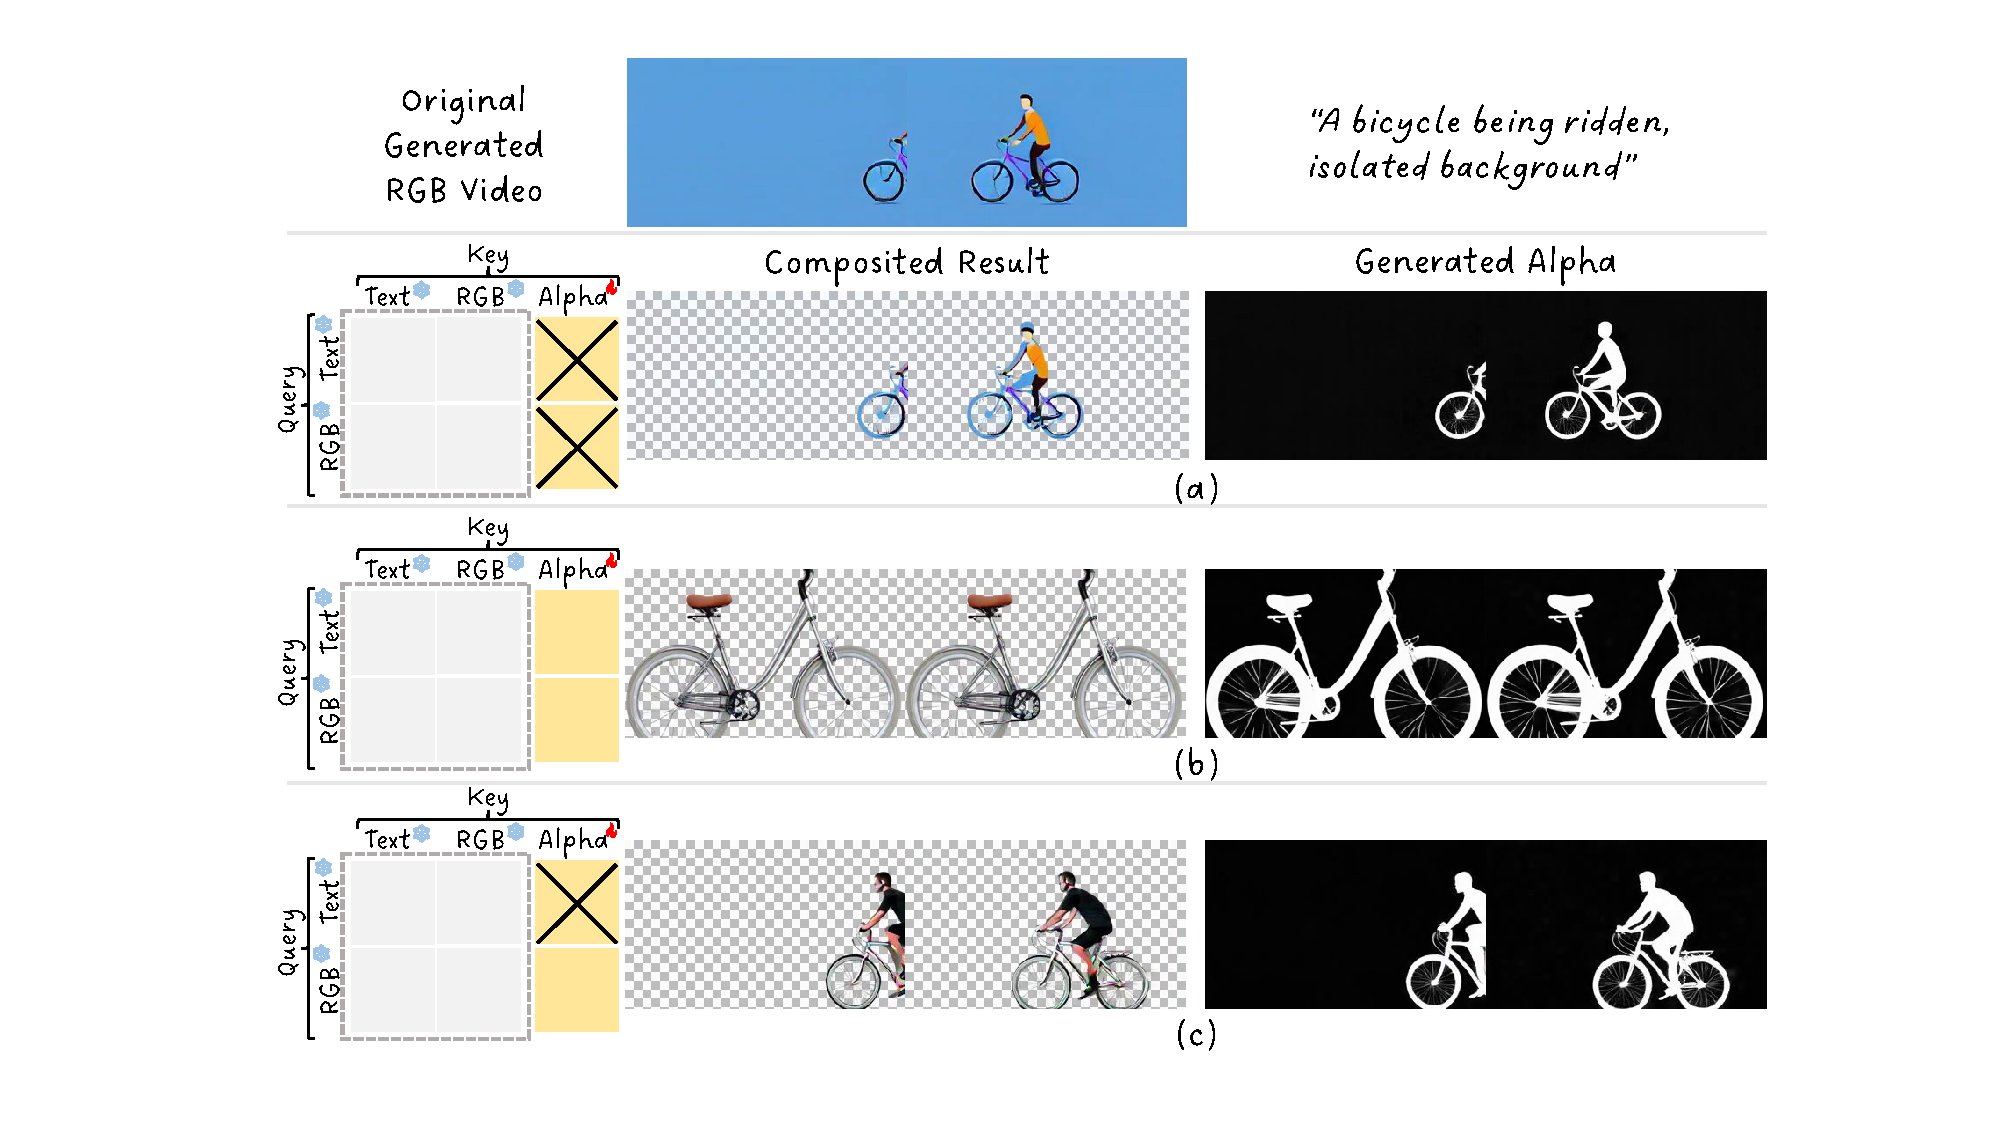
\includegraphics[width=1.0\linewidth]{figs/method-attn.pdf}
    \vspace{-0.2in}
    \caption{\textbf{Attention Rectification.} (a) Eliminating all attention from alpha as a key preserves 100\% RGB generation but leads to poor alignment. (b) Retaining all attention significantly degrades quality, causing a lack of motion in bicycles. (c) Our method achieves an effective balance.
    }
    \label{fig-attn}
    \vspace{-0.1in}
\end{figure}




%
% --- inline annotations
%
\newcommand{\red}[1]{{\color{red}#1}}
\newcommand{\todo}[1]{{\color{red}#1}}
\newcommand{\TODO}[1]{\textbf{\color{red}[TODO: #1]}}
% --- disable by uncommenting  
% \renewcommand{\TODO}[1]{}
% \renewcommand{\todo}[1]{#1}

\usepackage{xcolor}
\usepackage{graphicx}
\usepackage{booktabs}
\usepackage{amsmath} 
\usepackage{amsfonts}
\usepackage{amssymb}
\usepackage{multirow} 
\usepackage{makecell}
\newcommand{\shline}{\Xhline{1.1pt}} % Adjust thickness as desired

\section{Experiments}
\label{sec:experiments}

We present results for supervised video classification and self-supervised masked auto-encoding with frozen representations evaluated on two downstream tasks: video classification and point tracking. To analyse the memory capabilities of our model, we also include a reconstruction task of frames seen in the distant past. Using the same task, we study the generalisation capabilities to longer sequences than seen during training. We follow the ViT scaling configurations and, unless otherwise stated, we use the \textbf{B}ase version for our model for all our experiments. We specify the number of parameters for all models considered in our experiments, and we include in the supplementary material all the training hyperparameters and data augmentations used in all experiments.

\subsection{Supervised video classification}

\par \noindent \textbf{Datasets:}
We use large-scale real-world datasets for the supervised video classification task. Kinetics400~\citep{Carreira_2017_CVPR} contains 241,512 videos\footnote{Kinetics is a dynamic dataset (videos may be removed from
YouTube). Our current version has 241,512 videos, compared to 267,000 videos reported in~\cite{vivit}, so a decrease of almost 10\%, noticeable in the final performance.} across train, validation, and test splits, 10s-long (25fps), spanning 400 classes. This dataset is known to require modelling appearance for successful action recognition. To challenge our model's capability of understanding motion, we also use SSv2 dataset~\citep{goyal2017something}, which contains 220,847 shorter videos (2-6s long), sampled at 12fps, representing 174 classes. This dataset includes actions that differ in finer motion-related details, requiring a deeper temporal understanding, e.g. \textit{pouring something into something} vs \textit{pretending to pour something into something}. 

\par \noindent \textbf{Baselines:}
We use ViViT~\citep{vivit} as our main baseline. We consider the full self-attention version, which patchifies and flattens the entire video, prepends a video class token, then runs self-attention blocks. We also consider the factorised encoder version (ViViT FE), which runs a ViT image model over all the frames, and uses temporal self-attention blocks to integrate the information over time. Finally, we also consider a baseline that uses only LRU recurrent and MLP blocks, configured similar to VideoMamba~\cite{li2024videomambastatespacemodel}, i.e. it does not use self-attention blocks, denoted \textit{PureLRU}. Similar to ViViT, this model first patchifies and flattens the video, prepends a class token, then applies a sequence of recurrent blocks. All baselines use learnt spatio-temporal positional encoding, whereas the proposed \ssm\ uses only spatial positional encoding as the temporal dimension is implicitly modelled through its recurrence.


\par \noindent \textbf{Results:} We include results for training from scratch or using Imagenet pre-trained weights to initialise the weights of the ViT blocks. Figure~\ref{fig:baselines} shows a first comparison between \ssm\ and the above baselines, with all models being trained from scratch on supervised classification on SSv2. We consider the \textbf{S}mall version for all models as the larger \textbf{B}ase version shows stability issues when trained from scratch, as reported in other works as well~\cite{li2024videomambastatespacemodel,vivit}. As expected, the performance on this challenging dataset when training from scratch is far from SOTA, but it clearly shows that the proposed factorisation has superior video modelling capabilities compared to baselines, ViViT-S with full self-attention being the closest competitor. PureLRU's performance is very poor, which is in line with the findings of other works (\eg VideoMamba) who report that bidirectional (non-causal) processing of the input is needed for good performance. 

We report further results comparing against ViViT-B and ViViT-L with full self-attention when using Imagenet pre-trained weights; see Table~\ref{tab:ssv2} for SSv2 results and Table~\ref{tab:kinetics} for Kinetics400 results.
We can observe that our model achieves better performance compared to ViViT baselines on SSv2, but it is slightly below ViViT-L on Kinetics400. This result could reflect the difference between the two datasets mentioned above: outperforming ViViT-L on SSv2 suggests that \ssm\ is superior at modelling motion compared to ViViT, but on Kinetics where the appearance is enough for successful classification, both models are on par. We consider this to be a strong positive result for our model given that it has about 3x less parameters compared to ViViT-L and significantly lower FLOPs count and memory footprint as shown in Figure~\ref{fig:memory}.

\begin{figure}[t]
  \centering
  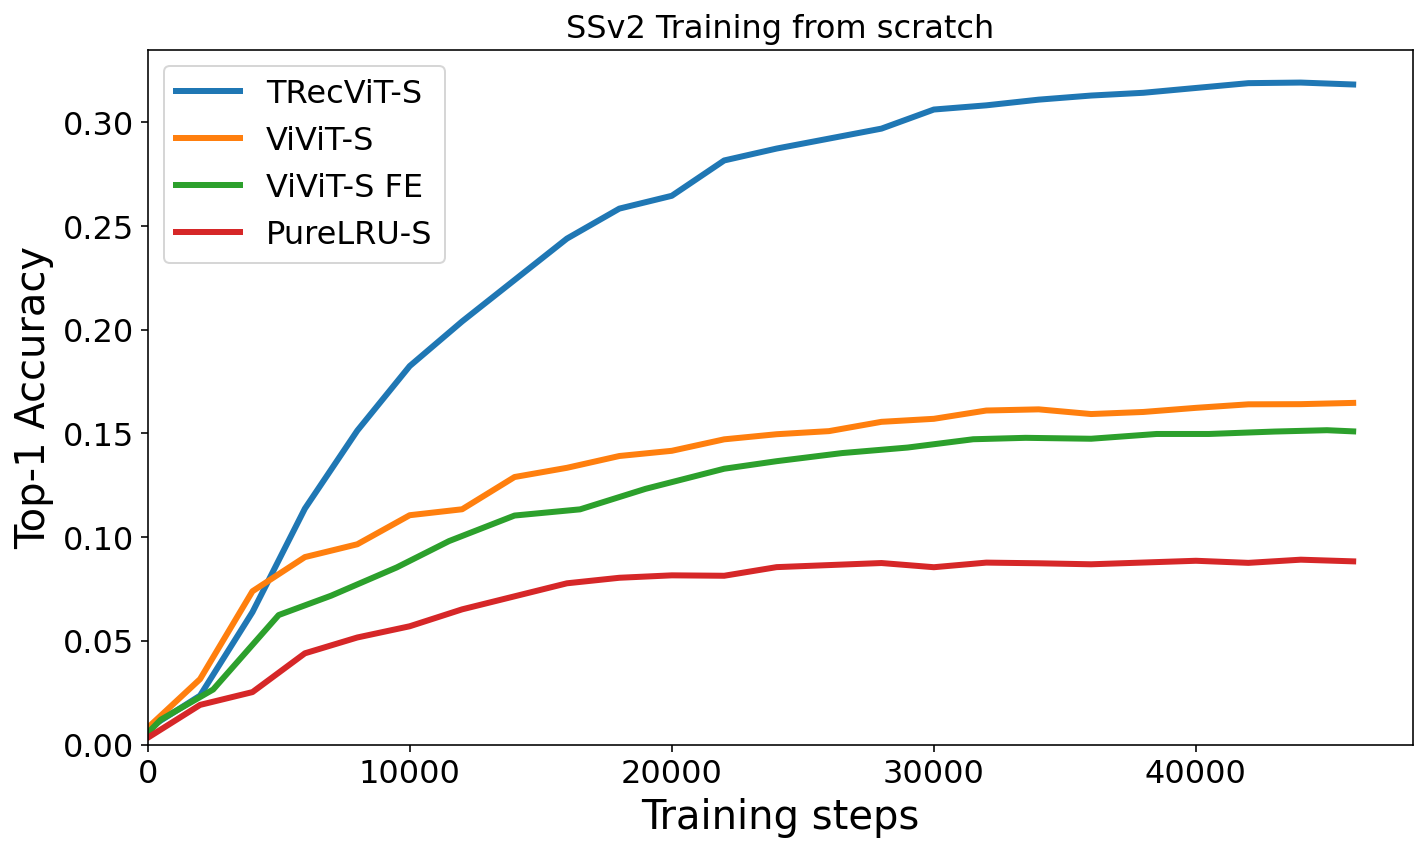
\includegraphics[width=.9\linewidth]{img/scratch.png}
  \caption{\ssm\ compared to baselines on supervised video classification on SSv2 dataset, trained from scratch. The plot shows the evolution of the evaluation accuracy as training progresses.
  }

  \label{fig:baselines}
\end{figure}
 

 \begin{figure*}[h]
  \centering
  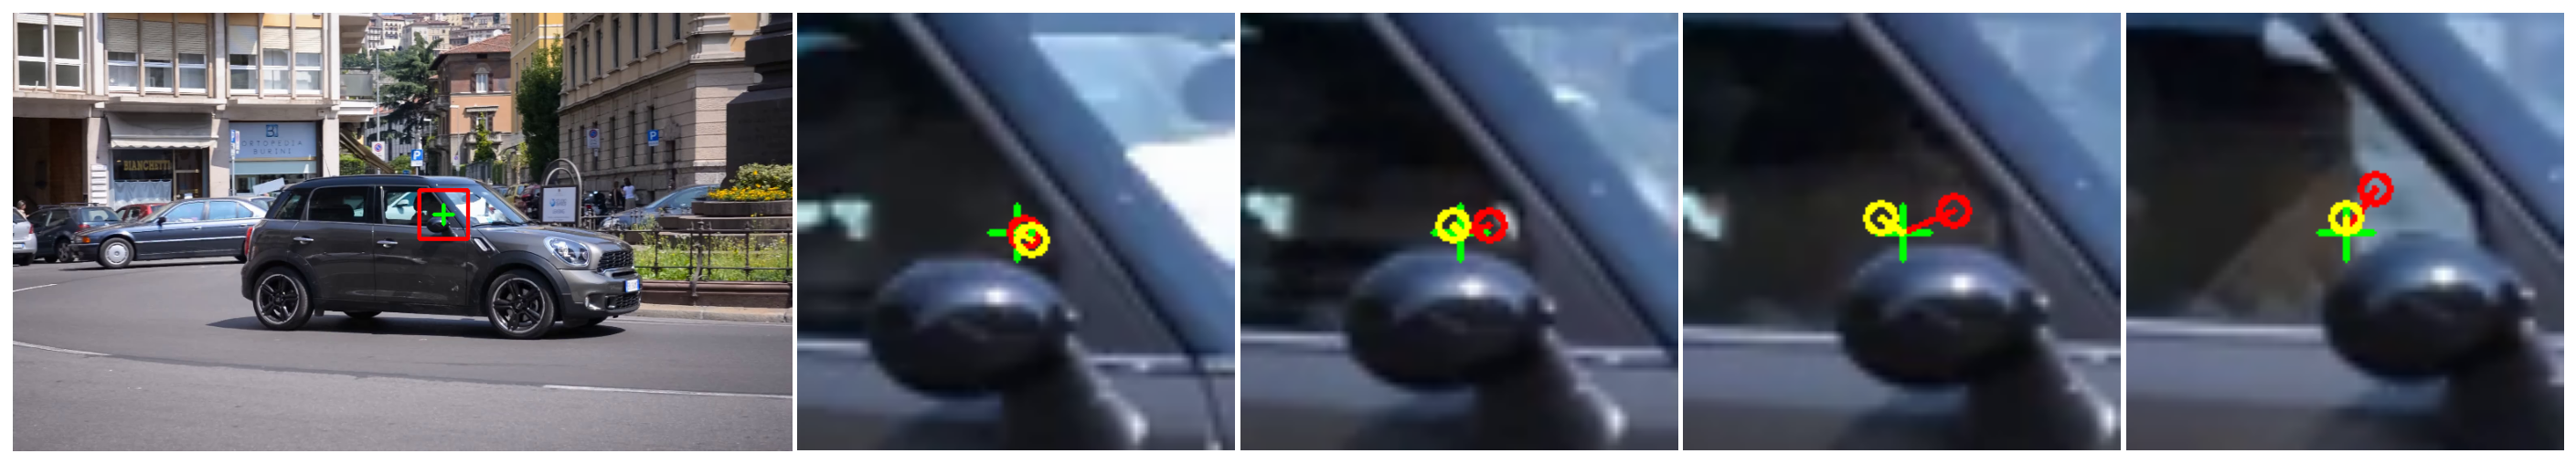
\includegraphics[width=\linewidth]{img/davis.png}
  \caption{Qualitative results obtained by \ssm\ for point tracking on DAVIS dataset compared to VideoMAE. The leftmost image indicates the point to track in the original frame, and the images towards the right show zoom-ins on subsequent frames. Green plus (+) marker indicates the ground truth, yellow circle indicates \ssm's predictions and red circles indicate VideoMAE's predictions.}
  \label{fig:tracking}
\end{figure*}


\begin{table}
    \centering
    \small{
    \begin{tabular}{l|c|c|r}
    \hline
    \textbf{Model} & \textbf{Patch size} & \textbf{Top-1 acc (\%)} & \textbf{\# params} \\
    \hline
    ViViT-B & (2, 16, 16) & 59.1 & 90M \\
    ViViT-L & (2, 16, 16) & 65.9 & 320M \\
    \ssm\ & (1, 16, 16) & \textbf{66.8} & 109M\\
    \hline
    \end{tabular}}
    \caption{Performance of \ssm\ compared to ViViT-B and ViViT-L baselines on SSv2 dataset with all models initialised from Imagenet pre-training. For ViViT-L, we use the result reported by its authors, for ViViT-B we obtained the results internally as they were not reported in the original paper for this dataset.}
    \label{tab:ssv2}
    \end{table}
    
\begin{table}
    \centering
    \small{
    \begin{tabular}{l|c|c|r}
    \hline
    \textbf{Model} & \textbf{Patch size} & \textbf{Top-1 acc (\%)} & \textbf{\# params} \\
    \hline
    ViViT-B & (2, 16, 16) & 78.1 & 90M \\
    ViViT-L & (2, 16, 16) & \textbf{78.7} & 320M \\
    \ssm\ & (1, 16, 16) & 78.4 & 109M\\
    \hline
    \end{tabular}}
    \caption{Performance of \ssm\ compared to ViViT-B and ViViT-L baselines on Kinetics400 dataset, with all models initialised from Imagenet pre-training. For ViViT-B and ViViT-L, we include the result we obtained internally by re-training the model on the current Kinetics400 dataset version; see footnote. In the original paper, the authors reported 80.3\% on Kinetics400 for ViViT-L.}
    \label{tab:kinetics}
    \end{table}

\subsection{Self-supervised masked autoencoding}
\label{sec:mae}
We use Kinetics400 for self-supervised pre-training from scratch and we report results on multiple downstream datasets and tasks by fine-tuning attention readout heads on top of frozen representations. We choose this setup, as opposed to fine-tuning end-to-end, as the  performance in this case more clearly reflects the quality of the pre-trained representations. As mentioned in the previous section, we use a large masking ratio (0.90), which makes pre-training very efficient. We report the number of parameters for every model considered. Note that the number of parameters for \ssm\ is different from the one reported in the previous section due to the addition of the readout heads.

\par \noindent \textbf{Video classification:}  We report video classification accuracy as downstream task using attention readout heads on SSv2 and Kinetics400. We compare the performance against VideoMAE-L~\cite{tong2022videomae} in Table~\ref{tab:selfsup}. Our model obtains slightly better performance on both datasets compared to this strong baseline, despite having almost 3$\times$ less parameters. 

\par \noindent \textbf{Point tracking:} To demonstrate that our model can handle dense(r) tasks as well, we evaluate the same frozen MAE representations for the point tracking task. We use the recurrent architecture in MooG~\cite{steenkiste2024moving} as a readout due to its simplicity. MooG uses light cross-attention layers to process the embeddings of each frame in order, and the readout state is carried over through time. We finetune the MooG readout head using MOVi-E dataset~\cite{movie} as done in popular point tracking works~\cite{DoerschYVG0ACZ23}. We evaluate these fine-tuned representations on two datasets: Perception Test~\citep{patraucean2023perception} and DAVIS dataset~\cite{davis2017} with point tracks extracted in~\cite{doersch2022tapvid}. We report average Jaccard metric~\cite{doersch2022tapvid} for \ssm\ compared with MooG and VideoMAE; see Table~\ref{tab:pt}. \ssm\ obtains better performance on both datasets compared to baselines, which reinforces the observation that our proposed model has strong motion modelling capabilities. We include qualitative results for this task in Figure~\ref{fig:tracking}. We can observe that the results are visibly better compared to VideoMAE. More visualisations are included in the supplementary material.

\begin{table}
    \centering
    \small{
    \begin{tabular}{l|c|c|r}
    \hline
    \textbf{Model} & \textbf{Dataset} & \textbf{Top-1 acc (\%)} & \textbf{\# params} \\
    \hline
    VideoMAE & Kinetics400 & 45.8 & 330M \\
    \ssm\ & Kinetics400 & \textbf{46.0} & 128M\\
    \hline
    \hline
    VideoMAE & SSv2 &  53.7 & 330M \\
    \ssm\ & SSv2 &  \textbf{53.9} & 128M\\
    \hline
    \end{tabular}}
    \caption{Performance of \ssm\ compared to VideoMAE on video classification using frozen MAE representations, pre-trained on Kinetics400.}
    \label{tab:selfsup}
    \end{table}

\begin{table}
    \centering
    \small{
    \begin{tabular}{l|c|c|c|r}
    \hline
    \textbf{Model} & \textbf{Dataset} & \textbf{\# frames} & \textbf{AJ} & \textbf{\# params} \\
    \hline
    MooG & DAVIS & 8 & 0.687 & 35M \\
    VideoMAE & DAVIS & 8 & 0.703 & 330M \\
    \ssm\ & DAVIS & 8 & \textbf{0.706} & 128M\\
    
    \hline
    \hline
    MooG & Perception Test & 16 & 0.760 & 46.5M \\
    VideoMAE & Perception Test & 16 & 0.761 & 330M \\
    \ssm\ & Perception Test & 16 & \textbf{0.783} & 128M\\
    \hline
    \end{tabular}}
    \caption{Performance of \ssm\ compared to baselines on point tracking task on DAVIS and Perception Test datasets. All models use frozen representations evaluated using the readout head from MooG.}
    \label{tab:pt}
    \end{table}

\begin{figure*}[h]
  \centering
  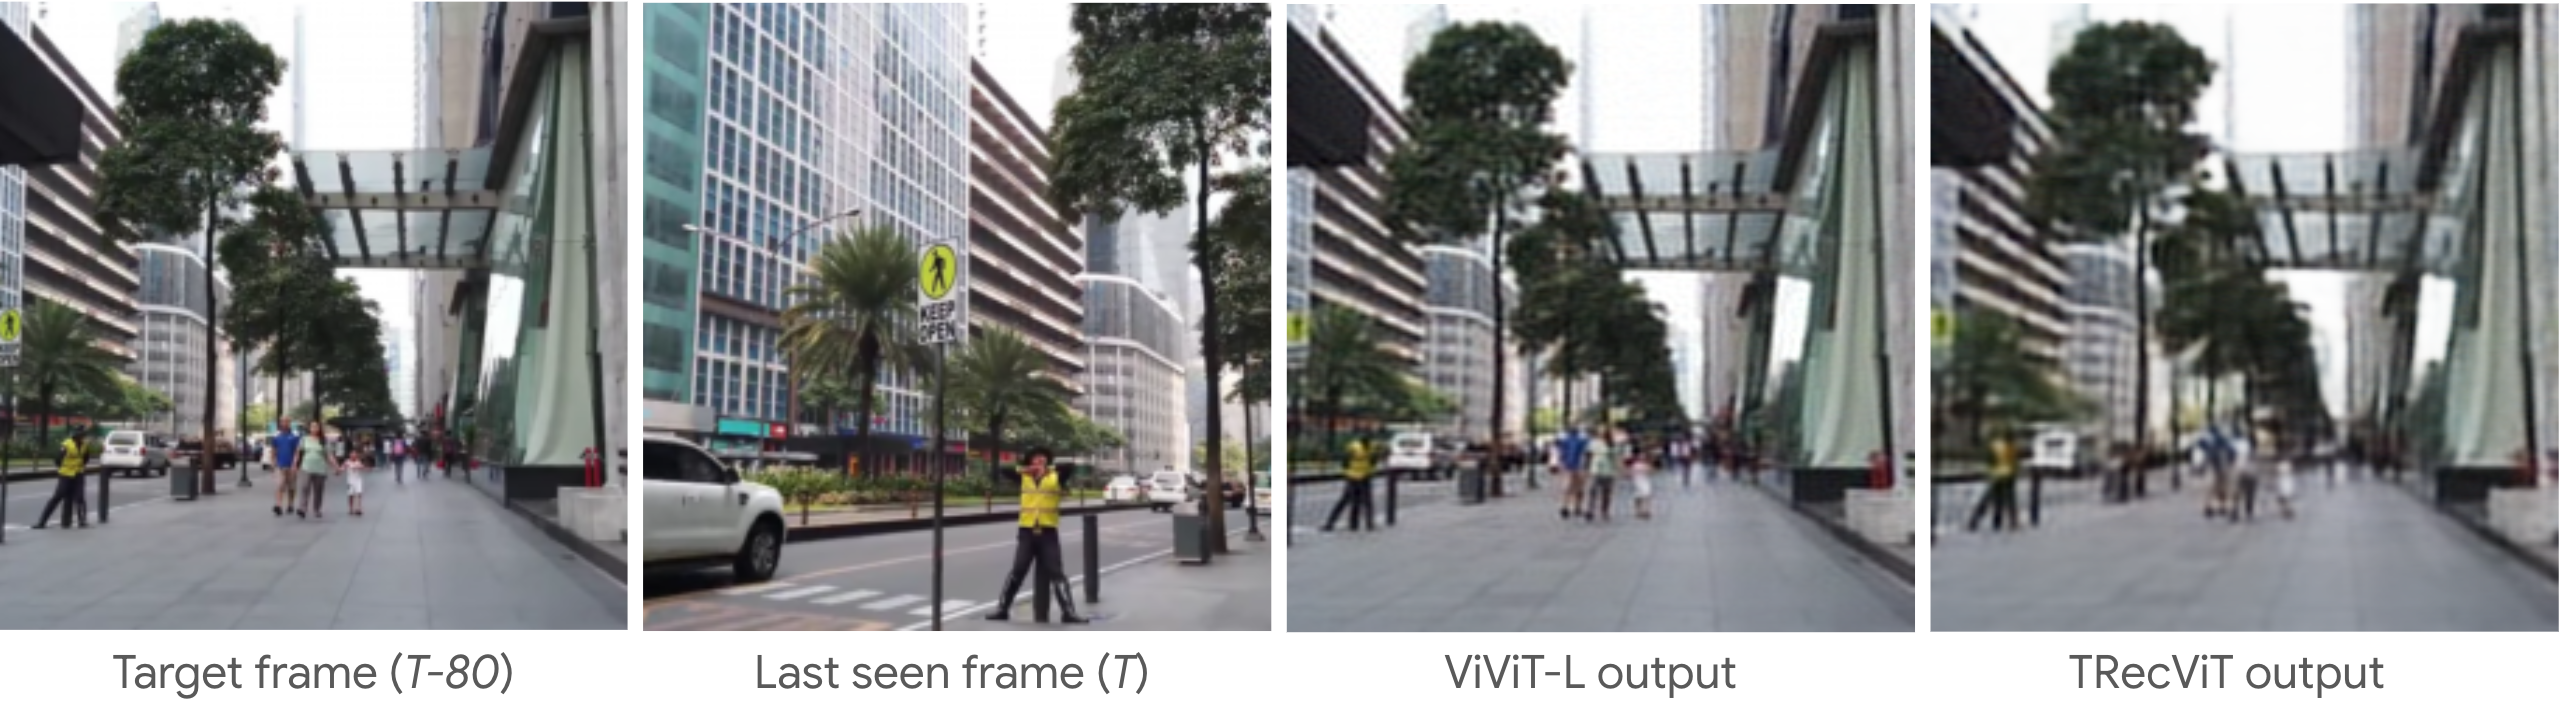
\includegraphics[width=\linewidth]{img/wtlong.png}
  \caption{Qualitative results obtained by \ssm\ on the dense memorisation task compared to ViViT-L. Both models are trained using Imagenet pre-trained weights, on video sequences of $T=64$ frames and they reconstruct the $(T-48)^\text{th}$ frame.}
  \label{fig:wt}
\end{figure*}

\begin{figure}[t]
\centering
\begin{subfigure}{0.48\linewidth}
    \centering
    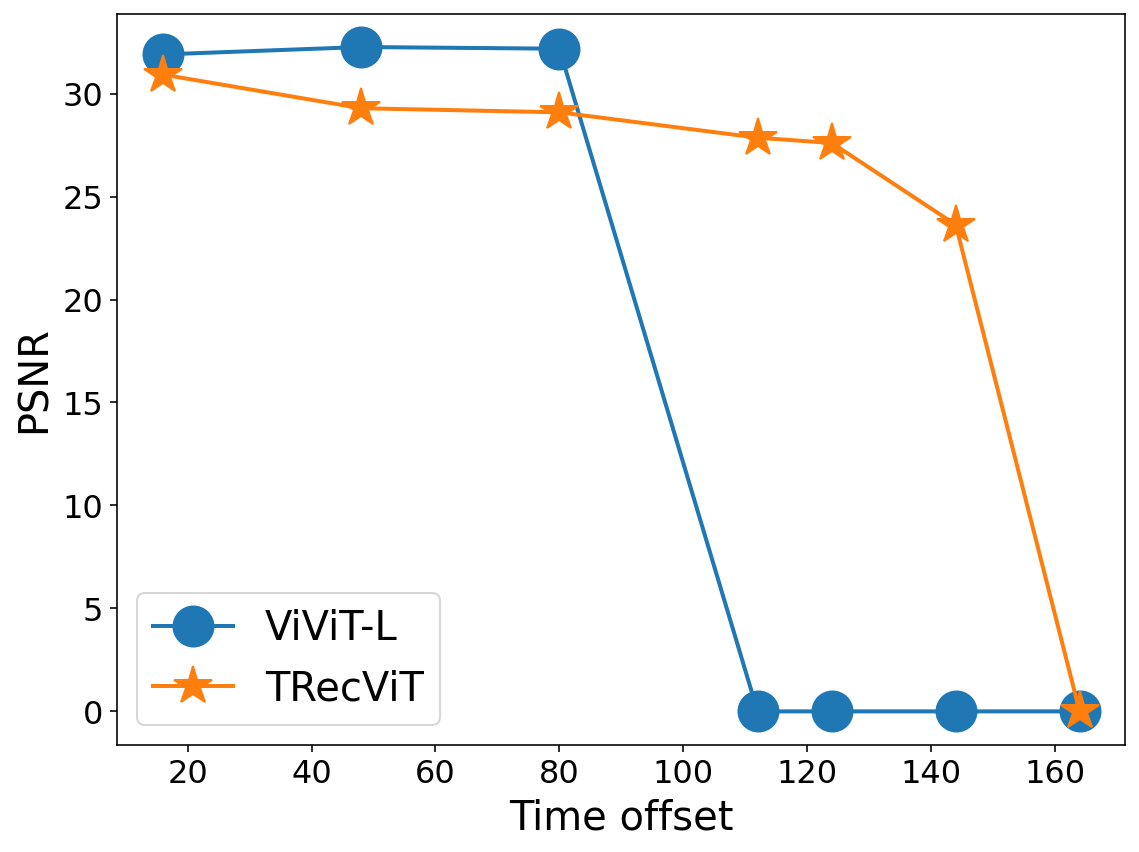
\includegraphics[width=\textwidth]{img/psnr.png}
    \caption{PSNR comparison}
\end{subfigure}%
\hfill
\begin{subfigure}{0.48\linewidth}
    \centering
    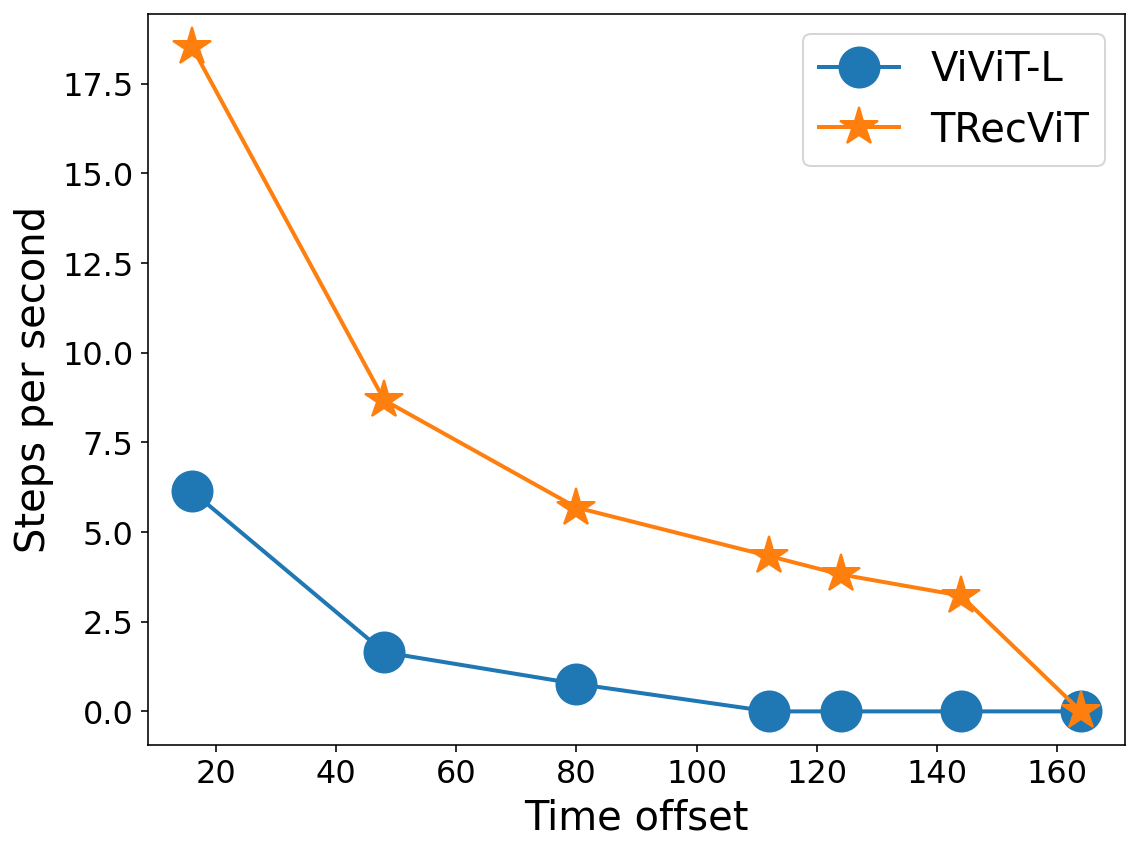
\includegraphics[width=\textwidth]{img/sps.png} 
    \caption{Steps-per-second comparison}
\end{subfigure}
\caption{Long video memorisation task. At time $T$, the model has to reconstruct the $(T-k)^\text{th}$ frame seen in the past. The plots show PSNR and throughput (steps-per-second) for increasing time offset $k$. For both models, the data points with $0$ value on the $y$-axis correspond to OOM.
}
\label{fig:psnr}
\end{figure}

\subsection{Long video memorisation task}
\label{sec:longtask}

Transformer models for language are known to be excellent at retrieving information from context, as they cache the keys and values for the entire history. On the other hand, LRUs / SSMs and RNNs in general struggle with such \emph{needle-in-the-haystack} style tasks as they need to perform the retrieval based on the compressed history kept in their recurrent state~\cite{jelassi2024repeat, de2024griffinmixinggatedlinear}. 
We are interested in studying this aspect in the video domain as well. We set up a simple reconstruction task where the model has to remember the frame seen at a given time-step in the past. For our analysis, we run multiple experiments where the model is tasked to reconstruct the $(T-k)^{\text{th}}$ frame from the past, with increasing value for $k\in\{16, 48, 80, 112, 144, 164\}$ frames. We employ Walking Tours dataset~\cite{venkataramanan2023imagenet}, which contains hour-long videos, and the scenery changes constantly, hence we are guaranteed that the video frames seen most recently will be very different compared to the frames seen earlier on. We scale the videos to $224\times224$ pixels. Again, we adopt ViViT-L as baseline, and we train both models using Imagenet pretrained weights. For ViViT-L, we keep all the outputs from all $T$ time steps and apply temporal pooling and a $1\times1$ convolution to get the expected shape for the reconstructed frame. For \ssm, we simply keep the output of the last layer at time step $T$ and reshape it to the expected shape. We show quantitative and qualitative results respectively in Figures~\ref{fig:psnr} and~\ref{fig:wt}. We can observe that there is a performance--efficiency trade-off at play for \ssm: its performance is slightly below ViViT's for shorter memory spans (16, 48, 80), but its efficiency (steps-per-second) is significantly higher. However, beyond 80 frames, ViViT-L goes out of memory, whilst \ssm\ continues to give decent results up to 144 frames, going out of memory towards 164 frames. Figure~\ref{fig:wt} shows qualitative results compared to the baseline for the case where the models have to remember the frame seen at $T-48$ in the past. We can observe that the quality of ViViT-L's reconstruction is good. For \ssm, whilst the overall structure (encoded in lower frequencies) is correct, it struggles to remember the high-frequency content of the image. This is to be expected due to the compression happening in the recurrent state of the model. However, given how different the last seen frame is from the target frame, we consider this to be a very promising result that warrants further investigation into the memorisation capabilities of our model, which we leave as future work.

\subsection{Generalisation to longer sequences}
\label{sec:gentask}

Using the same task as above, we analyse the generalisation capabilities to sequences longer than those used during training. Specifically, we train the models with sequences of length $T=64$ frames to reconstruct the $T-48$ frame, and evaluate them on longer sequences $T=96$ to reconstruct the same frame. The \ssm\ model can run on longer sequences without any modification. For the ViViT model, we need to adapt the positional encoding to accommodate longer sequences. We use interpolation to nearest neighbour to obtain the desired length; cubic interpolation led to worse results. The performance of \ssm\ degrades slightly, with PSNR going down from 29.3 (when evaluated on the same sequence length as in training $T=64$) to 26.4 when evaluated with $T=96$ frame sequences. ViViT's PSNR, however, drops significantly, from 32.3 when evaluated on the same sequence length, to 15.1 when evaluated on longer sequences. We include qualitative examples in Figure~\ref{fig:gentask} where we can observe that ViViT's output contains stronger artefacts compared to \ssm. 

\begin{figure}[h]
  \centering
  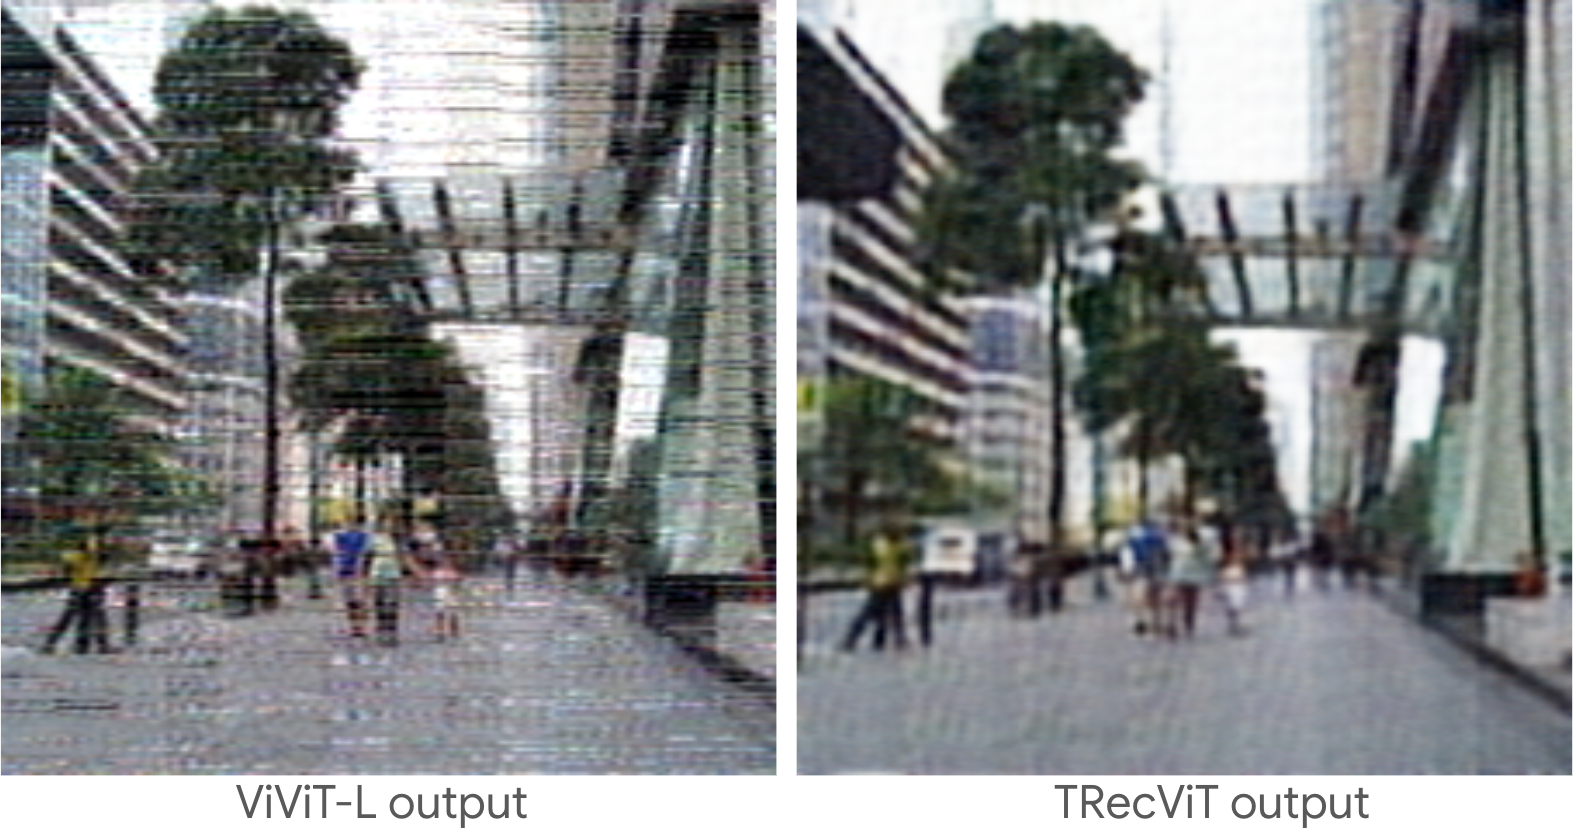
\includegraphics[width=\linewidth]{img/genlong.png}
  \caption{Generalisation to longer sequences. Both models are trained using Imagenet pre-trained weights, on video sequences of $T=64$ frames to reconstruct the $(T-48)^\text{th}$ frame; during evaluation, the models receive sequences of $T=96$ frames.}
  \label{fig:gentask}
\end{figure}

\section{Conclusion}
\label{sec:conclusion}
In this paper, we have investigated the common and unresolved issue that many established neural networks suffer from low floating-point operations per second (FLOPS). We have revisited a bottleneck operator, DWConv, and analyzed its main cause for a slowdown -- frequent memory access. To overcome the issue and achieve faster neural networks, we have proposed a simple yet fast and effective operator, PConv, that can be readily plugged into many existing networks. We have further introduced our general-purpose FasterNet, built upon our PConv, that achieves state-of-the-art speed and accuracy trade-off on various devices and vision tasks. We hope that our PConv and FasterNet would inspire more research on simple yet effective neural networks, going beyond academia to impact the industry and community directly.


\section*{Acknowledgements}
We would like to thank Caglar Gulcehre, Daniel Zoran, Dima Damen, and Andrew Zisserman for their insightful feedback throughout this project.
{
    \small
    \bibliographystyle{ieeenat_fullname}
    \bibliography{main}
}

% WARNING: do not forget to delete the supplementary pages from your submission 
\clearpage

\setcounter{page}{1}
\maketitlesupplementary

% \section{Supplementary video}
% Please see the supplementary video for an overview of our paper and for additional visualizations.

\section{\dataset Statistics}
We collected around 110k clips from 6,493 Internet VR180 videos.
\Fig{supp:camera_stats} shows the camera translation distribution between the first and last frame of each clip. 
In \Fig{supp:motion_stats}, we measure the motion in terms of pixel displacement projected onto the image frame. Measuring motion in pixel-space emphasizes motion that occurs closer to the camera, since such motion yields larger pixel displacements, while naturally de-emphasizing motion further from the camera. 

\section{More qualitative comparisons}
% Please see the supplementary video for additional visual examples of data in \dataset.


\subsection{More results on held-out  \dataset examples}
\Fig{supp:qualitative-stereo4d} shows additional \method predictions on the \dataset held-out test set, extending \Fig{result-wall-stereo4dtest} from the main paper. \Fig{supp:compare-stereo4d} shows additional qualitative examples of motion comparisons on \dataset test set, extending~\Fig{compare-stereo4d} from the main paper. \Fig{supp:compare-stereo4d} compares variants of DynaDUSt3R trained on different data sources. The model trained on PointOdyssey incorrectly predicts large 3D motions, while the model trained on Stereo4D makes more accurate motion predictions, closer to ground truth.

\begin{figure}[t]
    \centering
    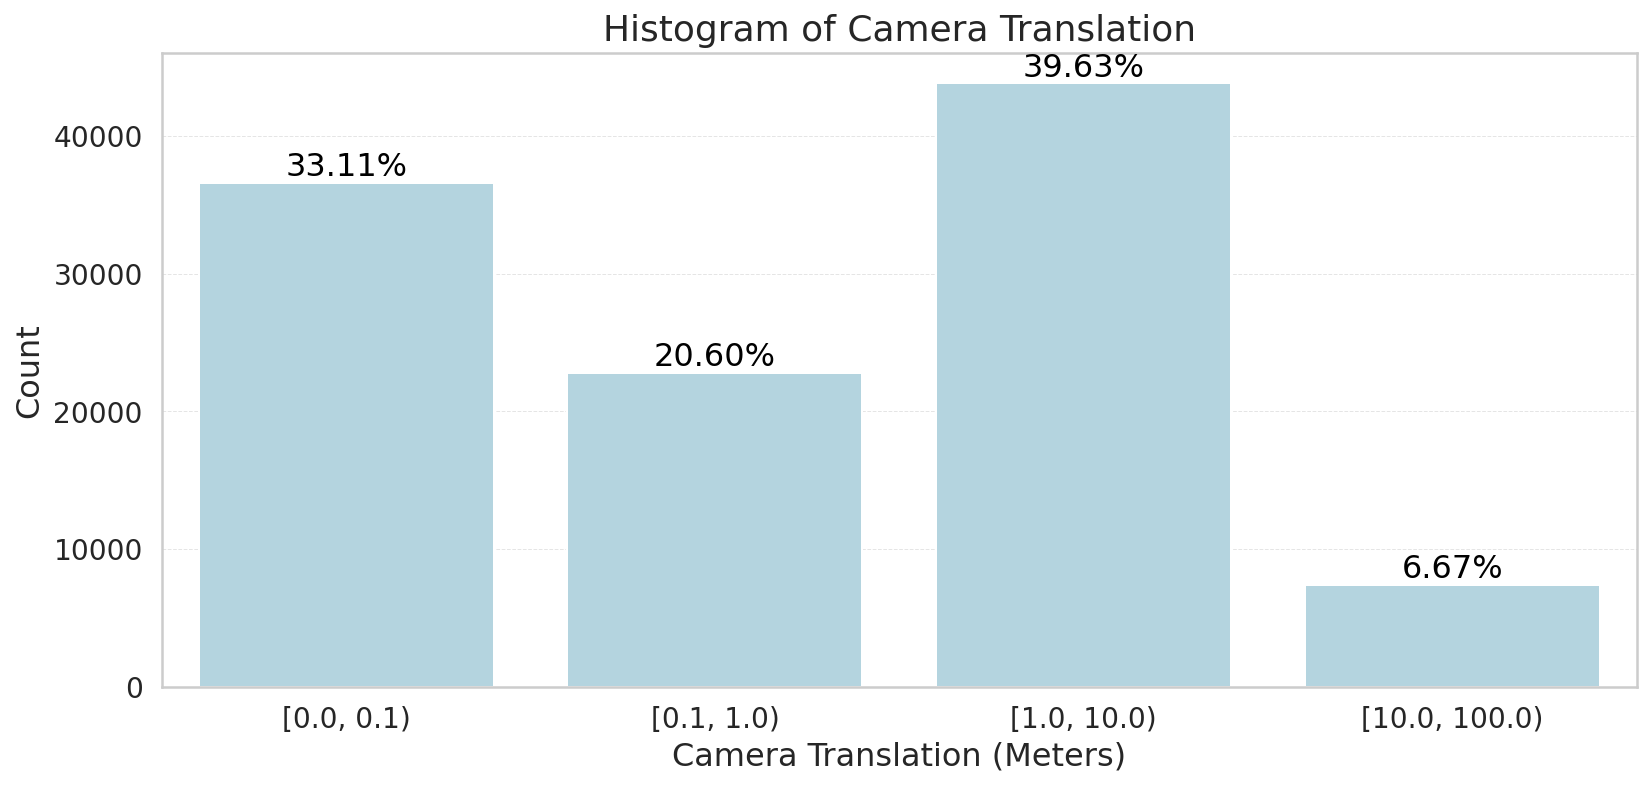
\includegraphics[width=\linewidth]{fig/supp/camera_stats.png}
    \caption{Camera statistics from \dataset. We measure the difference (in meters) of camera poses between the start and end frame of each video clip as calculated by SfM.}
    \label{fig:supp:camera_stats}

    \centering
    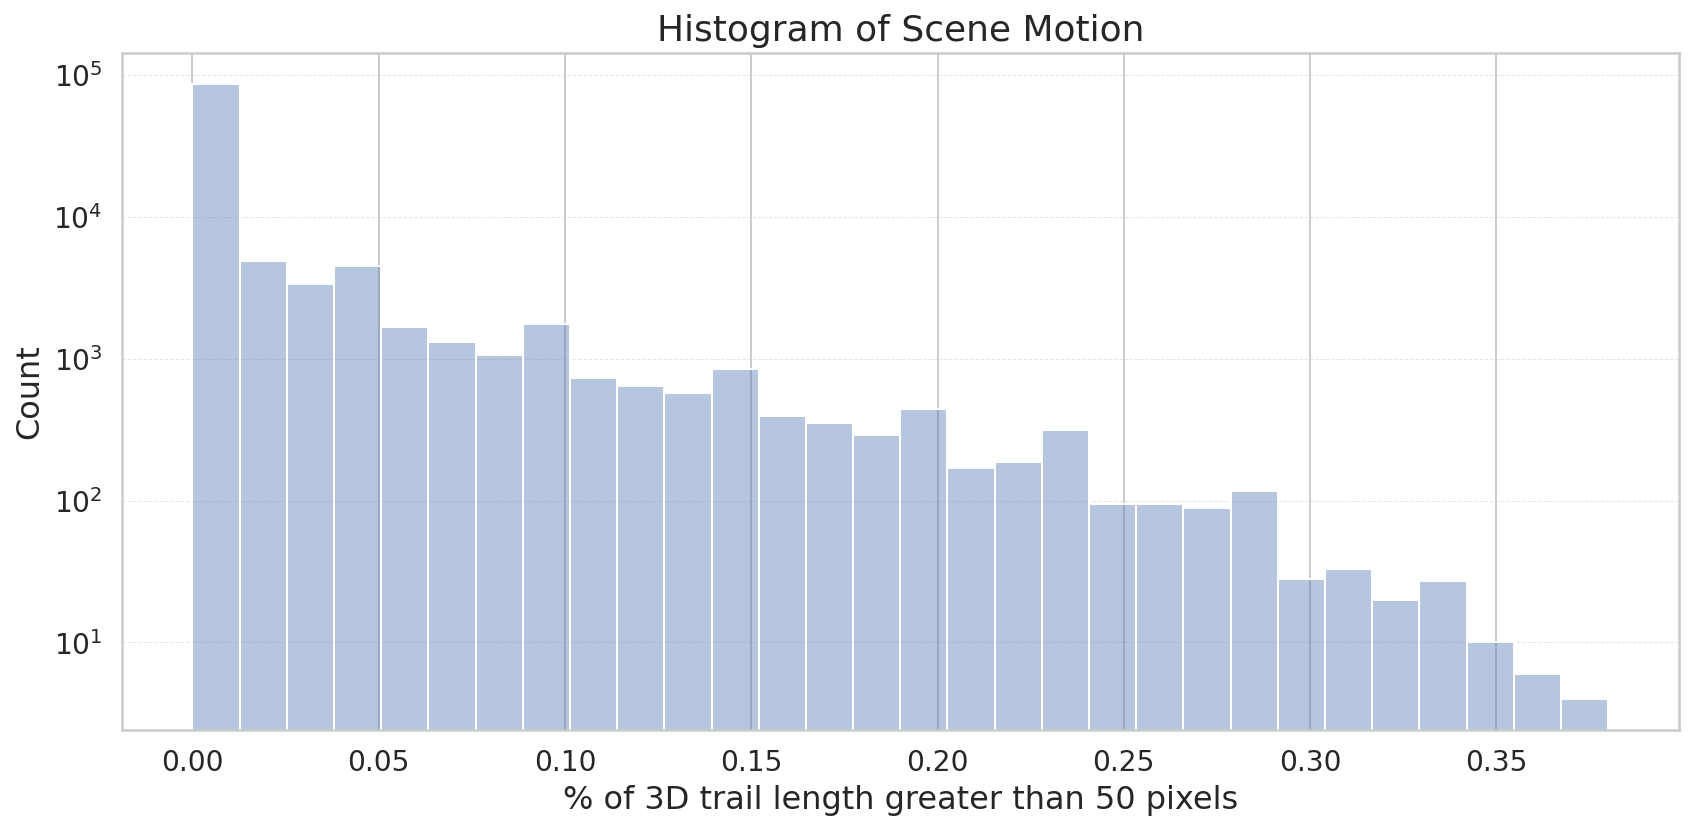
\includegraphics[width=\linewidth]{fig/supp/track_stats.png}
    \caption{Scene motion statistics from \dataset. We measure the motion in terms of pixel displacement projected onto the image frame. For each video, we measure the percentage of tracks that have 3D trail length greater than 50 pixels. The 3D trail length is measured by Eqn.~\ref{eqn:trail_length_def}. }
    \label{fig:supp:motion_stats}
\end{figure}

\begin{figure*}[ht]
    \centering
    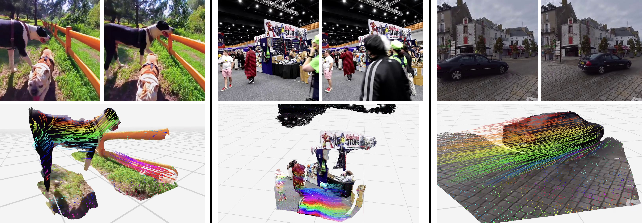
\includegraphics[width=\textwidth]{fig/supp/qualitative-stereo4d.pdf}
    \caption{\textbf{More qualitative results on \dataset test set.} Extending~\Fig{result-wall-stereo4dtest}, we visualize image pairs and corresponding dynamic 3D point clouds predicted by DynaDUSt3R trained on \dataset. Our method recovers accurate 3D shape and complex scene motion.}
\label{fig:supp:qualitative-stereo4d}
\end{figure*}

\begin{figure*}[ht]
    \centering
    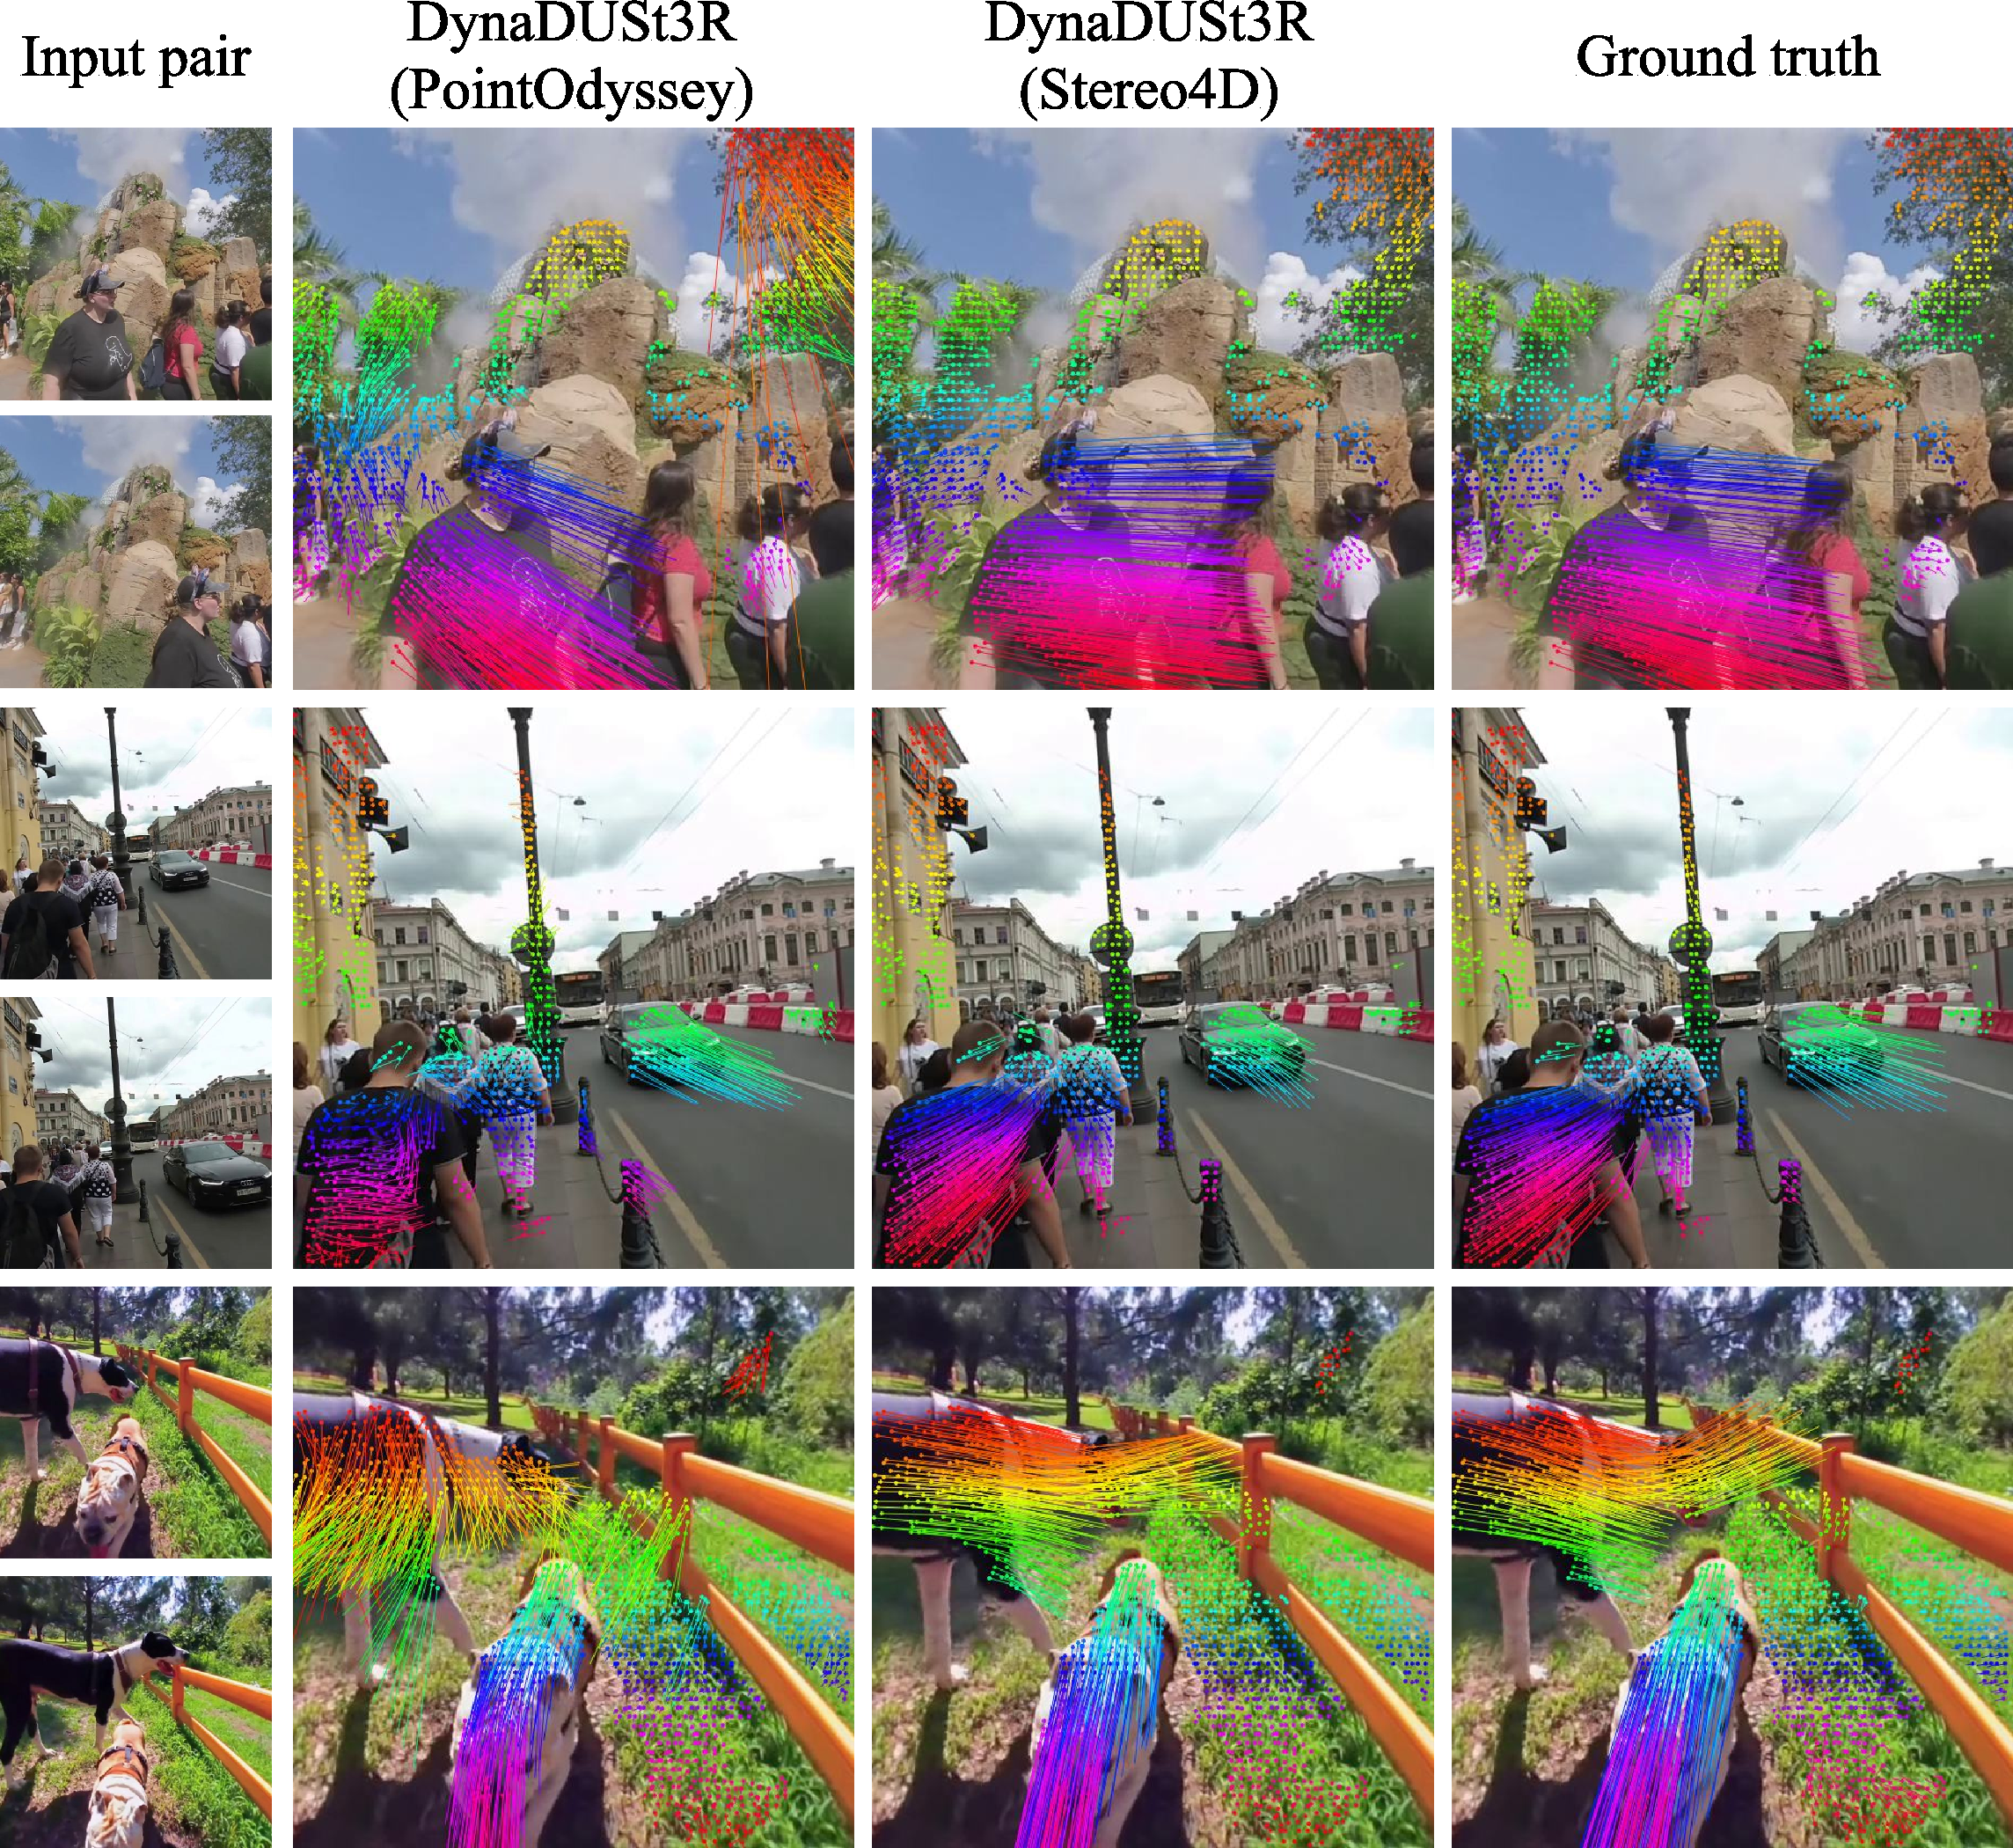
\includegraphics[width=\textwidth]{fig/supp/qualitative_comparison_on_motion_stereo4d.pdf}
    \caption{\textbf{More qualitative comparisons of 3D motion in the \dataset test set.} Extending~\Fig{compare-stereo4d}, we compare variants of DynaDUSt3R trained on different data sources. The Stereo4D-trained model also makes more precise motion predictions than the PointOdyssey-trained model.}
\label{fig:supp:compare-stereo4d}
\end{figure*}



\subsection{More qualitative examples on track optimization}
In \Fig{supp:track_comparison}, we illustrate estimated tracks for a video sequence featuring a forward-moving camera and vehicles driving towards the camera. Our initial 3D tracks derived directly from RAFT depth, BootsTAP 2D tracks, and SfM camera pose, show significant jitter for both dynamic (vehicle) and static (ground) points. 
However, after applying our track optimization, the ground points produce stable, static tracks, and vehicle tracks become smooth and coherent. 

\begin{figure*}[ht]
    \centering
    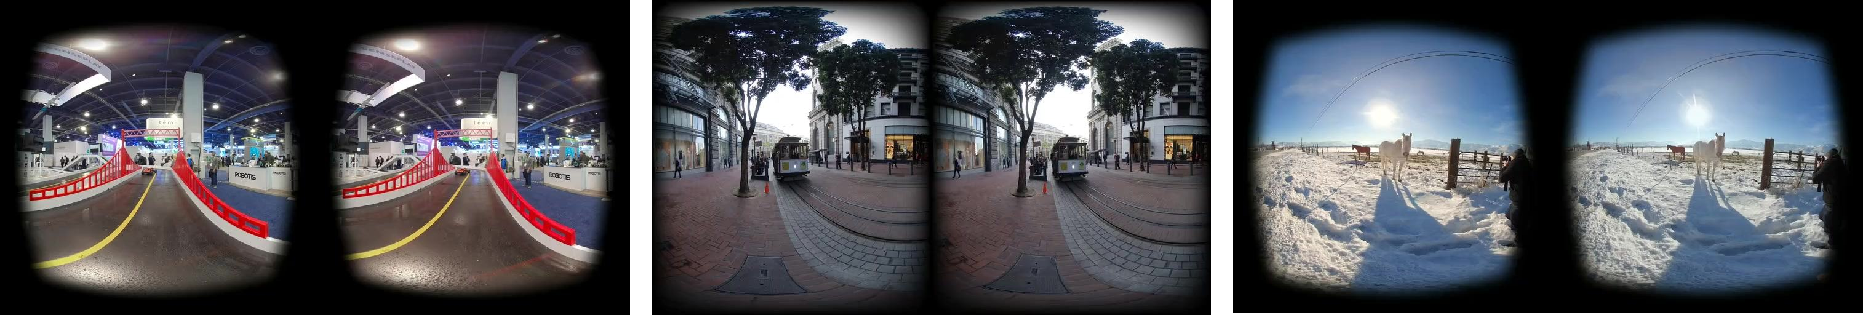
\includegraphics[width=\textwidth]{fig/supp/equirect-sample.pdf}
    \caption{Example equirectangular stereo videos collected from the internet.}
    \label{fig:supp:equirect}
\end{figure*}


\begin{figure*}[ht]
    \centering
    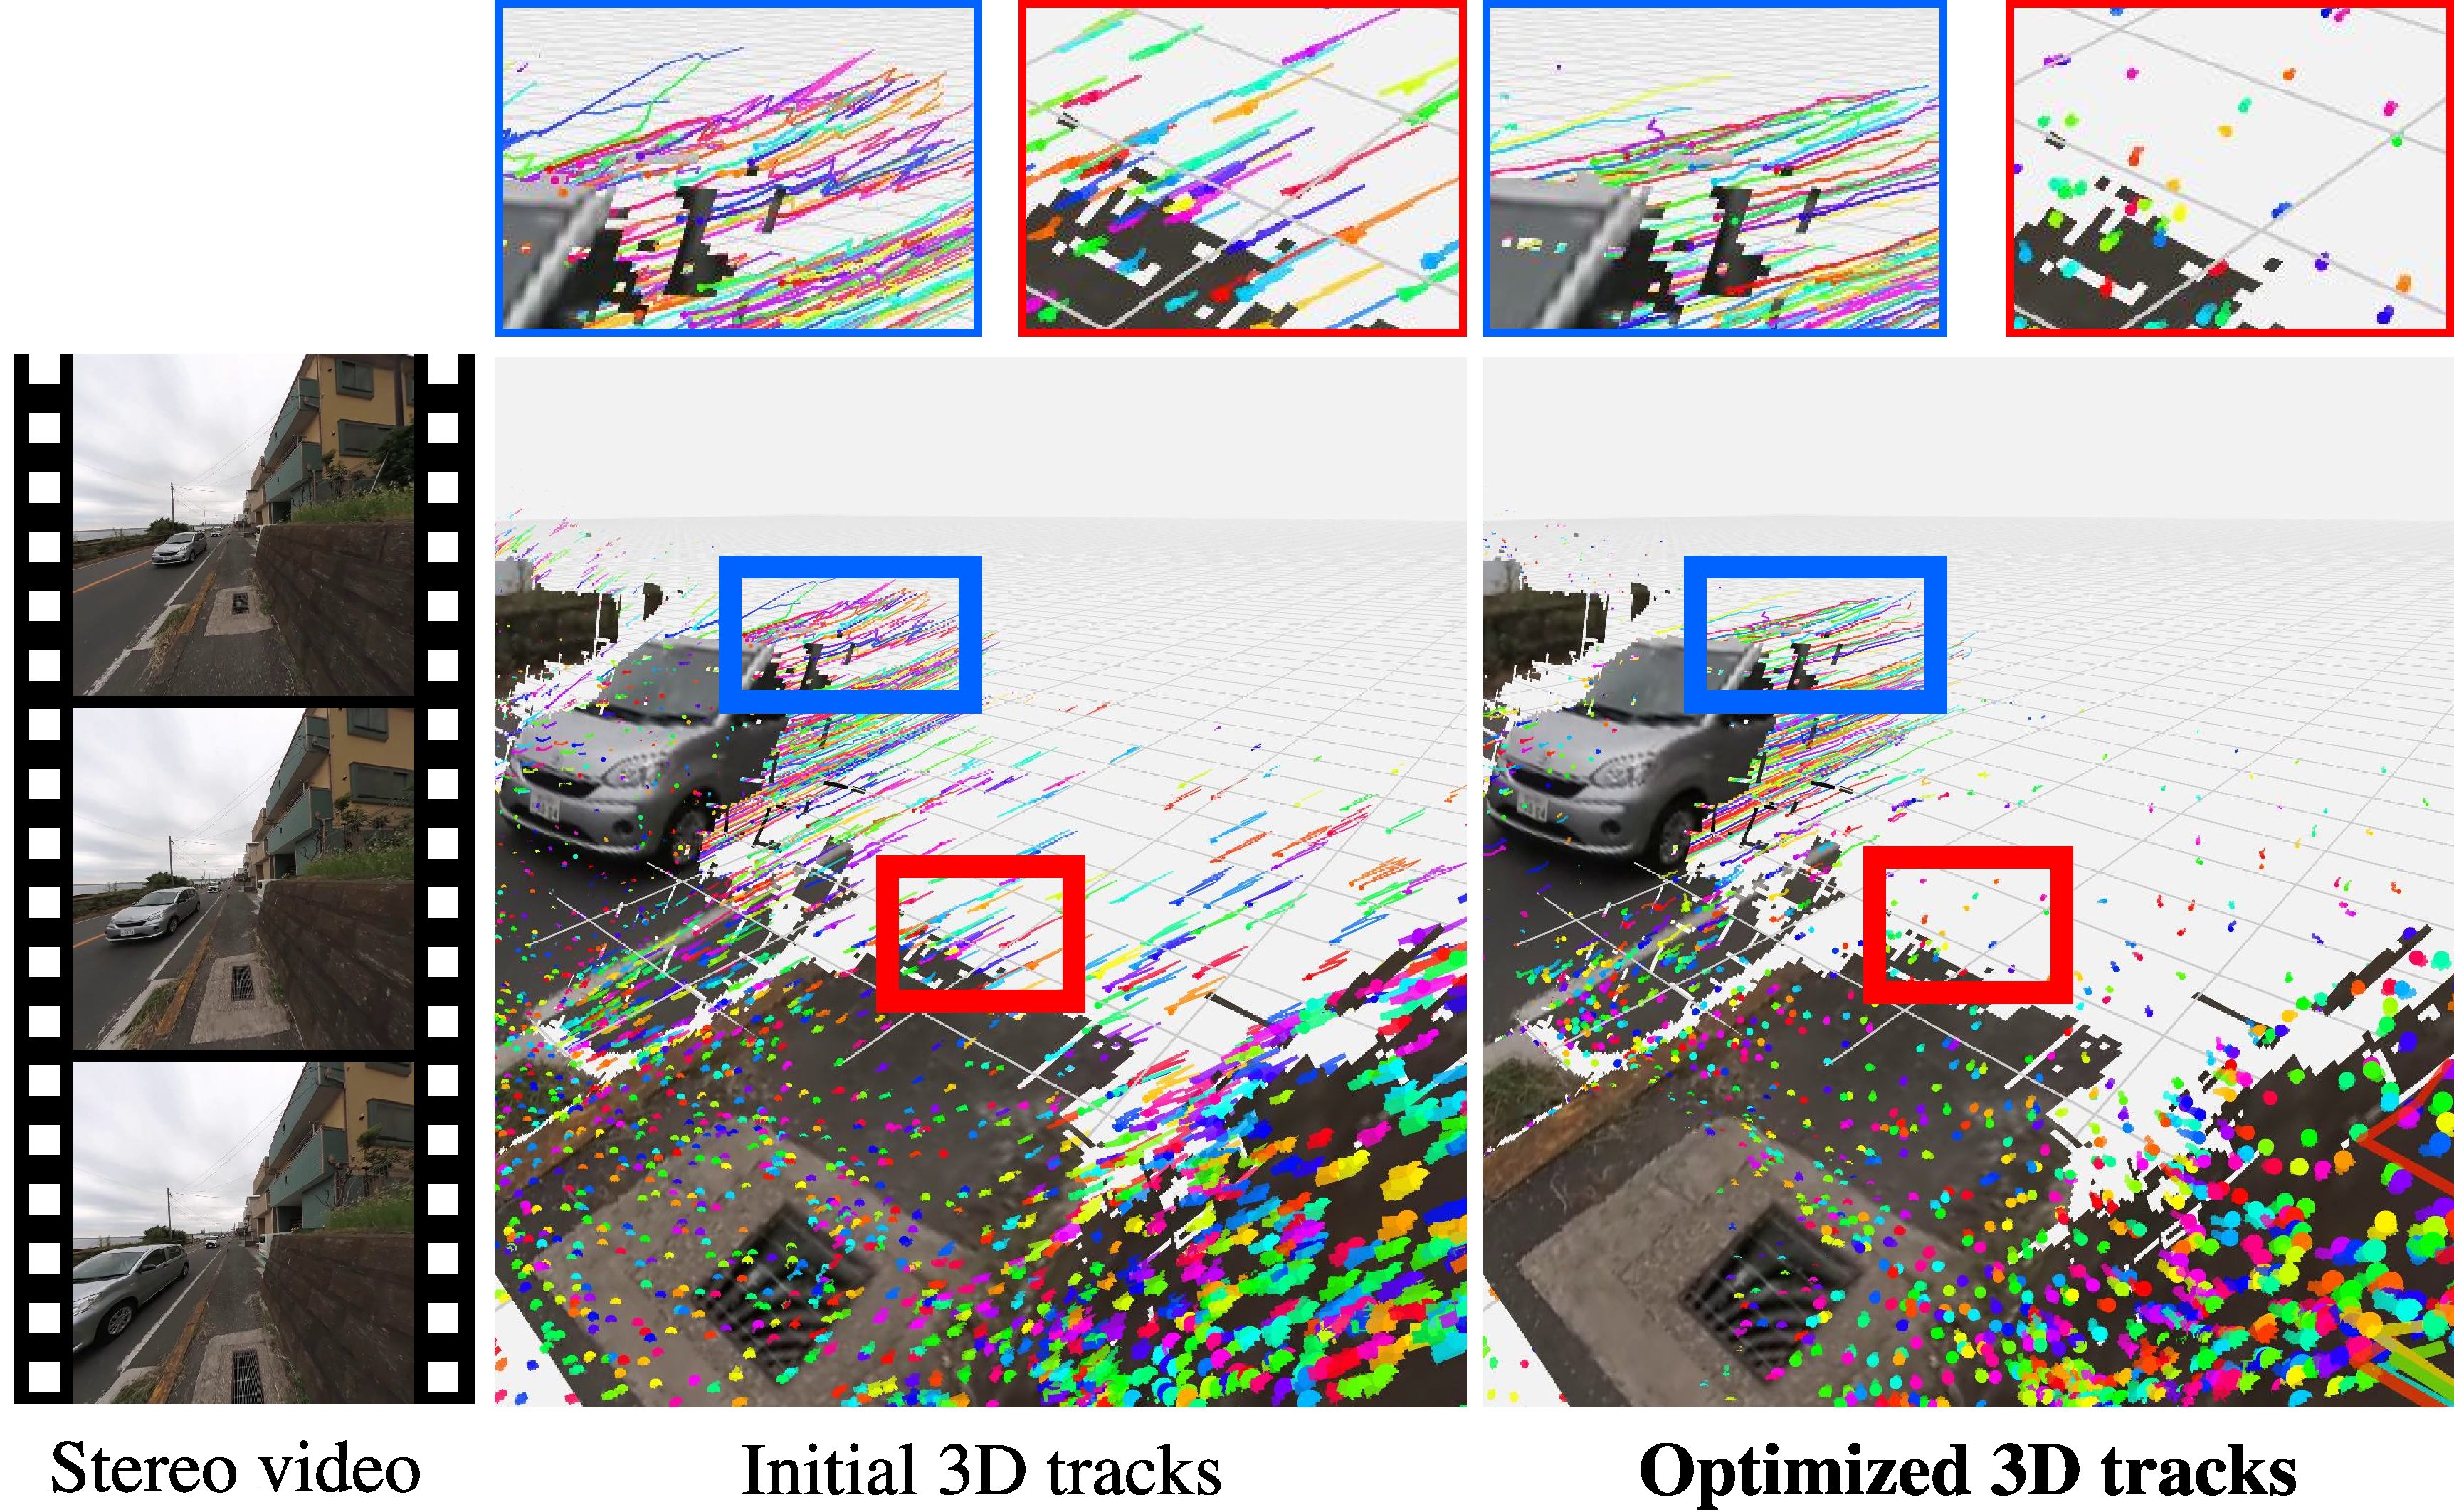
\includegraphics[width=0.8\textwidth]{fig/supp/track_optimization_car_comparison-2.pdf}
    \caption{\textbf{Effect of Track Optimization.} We compare 3D tracks on a challenging walking tour video sequence. In this clip (left), the camera moves forward while vehicles drive toward the camera. We visualize the results across 16 frames, showing 3D trails left by both dynamic and static points.  \textbf{Middle}: Our initial 3D tracks, created directly from RAFT, BootsTAP and SfM camera pose, also exhibit significant jitter for both dynamic (vehicle) and static (ground) points.  \textbf{Right}: After applying our track optimization, the ground points yield stable, static tracks, and vehicle tracks become smooth and coherent.}
\label{fig:supp:track_comparison}
\end{figure*}

\section{Dataset curation details}
\subsection{Equirectangular videos}
The raw videos that we collect (see examples in \Fig{supp:equirect}) are natively stored in a cropped equirectangular format, which differs from a full 360$^\circ$ equirectangular projection as the horizontal field of view of the cropped format typically spans 180$^\circ$---half of a full sphere. These videos often contain metadata specifying the horizontal and vertical field of view. 
For instance, metadata for a typical video might specify 
$\mathsf{start_{yaw}}=-90.0^\circ$, $\mathsf{end_{yaw}}=90.0^\circ$,  $\mathsf{start_{tilt}}=-90.0^\circ$, $\mathsf{end_{tilt}}=90.0^\circ$; 
Since many VR180 videos are designed for an immersive VR experience, they are typically viewed with headsets. Hence, the baseline between the left and right cameras typically closely matches the average human eye distance of 6.3 cm.


\subsection{SfM}
For ease of processing with standard 3D computer vision pipelines, and to benefit from the wide FoV of the input videos, we convert the videos from their native format (equirectangular projections) to a fisheye format for camera pose estimation. 
We use a 140$^\circ$ field of view for these fisheye-projected videos, because many equirectangular videos have a black fade-out/feathering/vignetting effect applied at the boundary, as shown in~\Fig{supp:equirect}.
We found that using wider FoV frames significantly improves camera pose estimation in dynamic scenes. 
When using narrow FoV projections, dynamic objects are more likely to occupy a large fraction of the frame; when these dynamic foreground objects are rich in features, they can confuse camera tracking algorithms, leading to inaccurate camera poses that track the dynamic object rather than producing true camera motion with respect to the environment. 
In contrast, wide-angle fisheye videos capture more background regions, which tend to have stable features for tracking, yielding more reliable camera poses.

We first use ORB-SLAM2's stereo estimation mode~\cite{murartal2015orbslam}
to identify trackable sequences within the videos, utilizing the method devised by Zhou \etal to divide videos into discrete, trackable shots~\cite{zhou2018stereo}. 
For each given shot, consisting of frames $(I_i, \ldots, I_n)$, we estimate camera poses and rig calibration via an incremental global bundle adjustment algorithm similar to COLMAP~\cite{schonberger2016structure}. 
We initialize the stereo rig calibration to be that of a rectified stereo pair with baseline 6.3 cm, but optimize for the calibration as part of the bundle adjustment process, as in practice the stereo rig can vary significantly from its nominal configuration.
This process yields a camera position $\mathbf{c}_i$ and orientation $\mathbf{R}_i$ for each frame $i$ (defined as the pose of the left camera), and a position $\mathbf{c}_r$ and orientation $\mathbf{R}_r$ for the right camera relative to the left (assumed to be constant throughout the shot).


\subsection{Depth estimation}
Depth estimation is first performed on a per-frame basis, with disparity maps computed independently for each frame.  

We use the estimated camera rig calibration $\cB_r, \RB_r$ to rectify the original  high resolution equirectangular video frames, ensuring that (1) the left and right views have centered principal points, (2) are oriented perpendicular to the baseline, and (3) pointing in a parallel direction.  We then convert the equirectangular videos to  perspective projections for downstream predictions.

Disparity is estimated from optical flow~\cite{teed2020raft, sun2022disentangling} between the rectified left and right frames. 
The $x$-component of the optical flow is used as disparity, which is converted to metric depth using:
\begin{equation}
    \mathsf{Depth} = \frac{\mathsf{baseline}  \times f}{\mathsf{disparity}}.
\end{equation}
Here $\mathsf{baseline}=0.063$m, and $f$ is the frame's focal length.

\medskip
\noindent \textbf{Outlier Rejection.} Several criteria are applied to filter out unreliable pixels: \emph{Inconsistency between left and right eyes:} Disparity is rejected if the optical flow fails a cycle-consistency check with an error exceeding one pixel. \emph{Depth values exceeding 20 meters} are considered invalid. Estimating accurate depth beyond a certain range requires sub-pixel disparity estimation, and therefore the resulting depths are usually very noisy.
\emph{Negative flow values} that shouldn't occur, but can, often due to errors in textureless regions.
\emph{Large vertical flow:} pixels with a y-component of flow exceeding one pixel are removed (as in our rectified stereo pairs correspondences should have the same $y$-value, and violating that epipolar constraint indicates uncertain matches).
\emph{Occlusion boundaries:} Depth gradients exceeding a threshold ($\mathsf{threshold} = 0.3$) indicate occlusion boundaries and are rejected. For a pixel location $(x, y)$, depth gradients are computed as:
$$\mathsf{grad_x}=|{\mathsf{Depth}(x+1, y)-\mathsf{Depth}(x-1,y)} |,$$ $$\mathsf{grad_y}=|{\mathsf{Depth}(x, y+1)-\mathsf{Depth}(x,y-1)} |.$$
Pixels are rejected if $\mathsf{grad_x} > \mathsf{threshold} \times \mathsf{Depth}(x,y)$ or  $\mathsf{grad_y} > \mathsf{threshold} \times \mathsf{Depth}(x,y)$.

\subsection{2D tracks}
We extract long-range 2D point trajectories using BootsTAP~\cite{doersch2024bootstap}. 
We run tracking on the left-eye video only. 
For every 10 frames, we uniformly initialize query points on image with stride 4. We then remove duplicated queries if earlier tracks fall within 1 pixel of a query point.

\subsection{Choice of FoV and resolution for perspective projection.}
When converting the equirectangular videos to perspective projections, we use two FoVs: 60$^\circ$ and 120$^\circ$. Both perspective videos are set to a resolution of $512\times512$, the maximum supported by BootsTAP. The 60$^\circ$ projection offers a higher sampling rate in scene units, which improves the accuracy of depth estimation and 2D tracks when measured in meters. Additionally, it has smaller perspective distortion near the image boundaries. In contrast, the $120^\circ$ projection provides wider coverage, ensuring longer 2D tracks across the videos. This trade-off allows us to balance data quality with spatial coverage for downstream tasks, e.g. \method. We take the union of the 3D tracks derived from each of these videos for \method training supervision.

\section{\method training details.}
\bfpar{Dataloader.} During training, we randomly sample two frames from the training videos that are at most 60 frames apart, at times $t_0$ and $t_1$, ($t_0 < t_1$). 
Additionally, we also sample one auxiliary frame in between, at time $t_{\mathsf{aux}}, t_0<t_\mathsf{aux}<t_1$, for additional track supervision between the two input frames. During training, we add data augmentation by applying random crops and color jitter to the input images and cropping the ground truth pointmap and motionmap accordingly. 

\bfpar{Training.} The network takes input the two RGB images as well as query times $t_q = \{0, 1, \frac{t_\mathsf{aux}-t_0}{t_1-t_0}\}$ and predicts the pointmaps for the two input views and motionmaps for each query $t_q$.
We supervise the network with losses defined in Eqn.~\ref{eqn:loss_point} and \ref{eqn:loss_motion}. We initialize our network with the \duster weights and initialize the motion head with the same weights as the point head. We finetune for 49k iterations with batch size 64, learning rate $2.5\times 10^{-5}$, and optimized by Adam with weight decay 0.95. 





\end{document}
